\documentclass[UTF8,zihao=-4]{ctexart}
\usepackage[a4paper,top=2.5cm,bottom=2.5cm,left=2.8cm,right=2.8cm,headheight=15pt]{geometry}
\usepackage{amsmath,amssymb,bm}
\usepackage{booktabs}
\usepackage{graphicx}
\usepackage{float}
\usepackage{array}
\usepackage{caption}
\usepackage{enumitem}
\usepackage{fvextra}
\usepackage{titlesec}
\usepackage{fancyhdr}
\usepackage{setspace}

\graphicspath{{figures/}}
\setlist[itemize]{leftmargin=2em}
\setlist[enumerate]{leftmargin=2em}
\captionsetup{
  font=small,
  labelfont=bf,
  labelsep=quad,
  skip=6pt
}
\renewcommand{\figurename}{图}
\renewcommand{\tablename}{表}
\renewcommand{\refname}{参考文献}
\numberwithin{equation}{section}
\setstretch{1.25}
\setlength{\parindent}{2em}
\setlength{\parskip}{0pt}
\setlength{\abovedisplayskip}{6pt}
\setlength{\belowdisplayskip}{6pt}
\setlength{\floatsep}{8pt plus 2pt minus 2pt}
\setlength{\textfloatsep}{10pt plus 2pt minus 2pt}
\setlength{\intextsep}{8pt plus 2pt minus 2pt}
\pagestyle{fancy}
\fancyhead{}

\fancyfoot[C]{\thepage}
\renewcommand{\headrulewidth}{0pt}
\renewcommand{\footrulewidth}{0pt}
\titleformat{\section}{\centering\heiti\zihao{3}}{\chinese{section}、}{0pt}{}
\titlespacing*{\section}{0pt}{1.2\baselineskip}{0.8\baselineskip}
\titleformat{\subsection}{\heiti\zihao{4}}{\arabic{section}.\arabic{subsection}}{0.8em}{}
\titlespacing*{\subsection}{0pt}{0.8\baselineskip}{0.4\baselineskip}
\renewenvironment{abstract}
{\begin{center}\heiti\zihao{4} 摘\quad 要\end{center}\zihao{-4}\setlength{\parindent}{2em}}
{\par\vspace{0.8\baselineskip}}
\fvset{
  fontsize=\scriptsize,
  breaklines=true,
  breakanywhere=true,
  numbers=left,
  numbersep=6pt,
  frame=single,
  framesep=2mm,
  tabsize=2
}

\title{基于回归分析与风险优化的 NIPT 检测时点选择及胎儿异常判定}
\author{}
\date{}
\makeatletter
\renewcommand{\maketitle}{
  \begin{center}
    \vspace*{0.5\baselineskip}
    {\heiti\zihao{2}\@title\par}
    \vspace{1.2\baselineskip}
  \end{center}
}
\makeatother

\begin{document}
\maketitle

\begin{abstract}
\noindent

无创产前检测（NIPT）的可靠性与胎儿 DNA 浓度、孕周、孕妇 BMI 及测序质量等因素密切相关。本文基于题目附件中男胎 1082 条、女胎 605 条检测记录，围绕男胎 NIPT 检测时点选择和女胎异常判定问题，建立相关回归、BMI 分组优化、多因素误差修正和综合异常评分模型。

针对问题一，本文将孕周数值化后，分析 Y 染色体浓度与孕周、BMI、年龄、体重等变量的关系。结果表明，Y 染色体浓度与孕周显著正相关，与 BMI、年龄和体重显著负相关。进一步建立含孕周、BMI 及交互项的回归模型，模型整体显著，但决定系数较低，说明该模型适合刻画总体变化趋势，个体浓度仍存在较明显波动。

针对问题二，本文以孕妇平均 BMI 为主要依据进行有序分组，并构造由时间风险和不达标惩罚组成的总风险函数。结果将男胎孕妇分
为 4 个 BMI 区间，其中 BMI 低于 30.05 的前三组推荐 10 周检测，高 BMI 组推荐 12.29 周检测。蒙特卡洛扰动和参数灵敏度分析表明，该分组结果在问题二设定下较稳定。

针对问题三，本文进一步引入年龄、孕情、妊娠方式和测序质量指标，并用正态误差描述检测波动，在达标比例约束下重新优化检测时
点。结果显示，前三个 BMI 组推荐时点后移至 12.86 周，高 BMI 组推荐 25 周，说明多因素修正和检测误差会提高过早检测的不达标风险，且结果对达标比例约束和误差水平较敏感。

针对问题四，本文以女胎非整倍体标记构造异常标签，综合染色体 Z 值、GC 含量偏离和读段质量风险建立异常评分。Youden 主阈值下模型准确率为 0.653，偏召回阈值可将召回率提升至 0.910。结果表明，该方法可作为低漏判倾向的辅助筛查工具，但不能替代临床诊断。


\textbf{关键词：}无创产前检测；Y 染色体浓度；BMI 分组；风险最小化；综合异常评分
\end{abstract}
\pagebreak
\section{问题重述}

\subsection{问题背景}

无创产前检测（Non-invasive Prenatal Testing, NIPT）通过采集孕妇外周血并检测其中的胎儿游离 DNA，对胎儿染色体异常风险进行筛查。母体血浆中胎儿游离 DNA 的发现为无创产前筛查提供了分子基础，高通量测序技术进一步推动了胎儿染色体非整倍体筛查的临床应用\cite{lo1997,bianchi2014}。与传统侵入式检查相比，NIPT 对孕妇和胎儿的直接损伤较小，已成为产前筛查中的重要技术手段。检测结果的可靠性与胎儿游离 DNA 在母体血浆中的比例密切相关；若胎儿 DNA 浓度过低，测序信号不足，可能导致检测失败或判断不稳定\cite{hui2020,deng2022}。

对男胎样本而言，Y 染色体浓度可作为胎儿 DNA 含量的重要表征。题目指出，当男胎 Y 染色体浓度达到 4\% 及以上时，检测结果通常具有较高可靠性\cite{contest2025c}。既有研究表明，胎儿 DNA 比例会受到孕周、孕妇体型、妊娠特征和实验测序因素共同影响\cite{hui2020,deng2022}。因此，如何根据孕周、BMI 及其他孕妇个体因素判断 Y 染色体浓度的变化规律，并选择合适的 NIPT 检测时点，是男胎检测策略优化的关键。

检测时点的选择存在明显权衡：若检测过早，Y 染色体浓度可能尚未达标，带来检测失败或重复检测风险；若检测过晚，即使检测结果更稳定，也可能缩短后续诊断和干预窗口，增加孕妇和胎儿的潜在风险。孕妇 BMI、年龄、孕情及测序质量等因素还会影响检测浓度和误差水平，使统一检测时点难以兼顾不同群体。

对女胎样本而言，由于不存在 Y 染色体浓度这一直接指标，异常判定需要综合 13、18、21 号染色体及 X 染色体的 Z 值、GC 含量、读段数和比例等测序指标。题目给出的女胎异常标签来自“染色体的非整倍体”字段，异常样本数量相对较少，因而女胎异常判定不仅要关注总体准确率，也需要重视漏判和误判之间的平衡。

\subsection{问题提出}

题目提供了男胎检测数据和女胎检测数据，要求围绕 NIPT 检测时点选择和胎儿异常判定完成以下建模任务。

第一，针对男胎样本，分析胎儿 Y 染色体浓度与孕妇孕周、BMI 等指标之间的相关关系，建立能够描述 Y 染色体浓度变化规律的统计模型，并检验相关变量及整体模型的显著性。

第二，在临床实践中 BMI 是影响男胎 Y 染色体浓度达标时间的重要因素。需要以 BMI 为主要分组依据，对男胎孕妇进行合理分组，并为每个 BMI 组确定一个最佳 NIPT 检测时点，使孕妇潜在风险尽可能小。同时，需要分析检测误差对分组结果和推荐时点的影响。

第三，在问题二仅考虑 BMI 的基础上，进一步综合孕妇身高、体重、年龄、怀孕次数、生产次数、妊娠方式、测序质量以及检测误差等因素，重新建立更完整的男胎 Y 染色体浓度达标概率模型。需要在保证各组达标比例的约束下，修正 BMI 分组和推荐检测时点，并与问题二结果进行比较。

第四，针对女胎样本，由于无法使用 Y 染色体浓度判断检测可靠性，需要综合考虑 X 染色体、13 号、18 号、21 号染色体的 Z 值，GC 含量，测序读段数及相关比例，BMI 等因素，建立女胎染色体异常的判定方法，并给出模型评价结果。

\section{问题分析}

\subsection{总体分析}

本题的四个问题具有由浅入深的递进关系。问题一侧重解释男胎 Y 染色体浓度与影响因素之间的统计关系，为后续达标概率和检测误差建模提供基础；问题二将问题一得到的浓度预测关系转化为不同 BMI 群体的检测时点决策；问题三在问题二的框架中加入个体协变量和检测误差，使推荐时点更加稳健；问题四则转向女胎异常判定，需要在缺少 Y 染色体浓度指标的情况下构造综合筛查规则。

从数据结构看，同一孕妇可能存在多次检测记录。若直接把所有检测记录用于分组优化，重复检测次数较多的孕妇会获得更高权重，影响 BMI 分组和达标比例估计。因此，本文在关系模型估计中使用记录层数据，以充分利用多次检测信息；在问题二、三的分组和风险优化中，则转化为孕妇层数据，使用每名孕妇的平均 BMI 和固定协变量计算组内达标比例。

从建模目标看，本题不是单纯追求拟合精度，而是要将统计关系转化为可执行的检测策略。因此，本文将模型分为两类：一类是解释和预测 Y 染色体浓度的回归模型，另一类是面向决策的风险优化模型。前者回答“哪些因素影响检测可靠性”，后者回答“不同 BMI 群体应何时检测”。女胎部分则采用综合评价和阈值判定思想，回答“在缺少 Y 染色体信息时如何辅助判断异常”。

\subsection{问题一的分析}

问题一需要研究男胎 Y 染色体浓度与孕周、BMI 等变量之间的关系。根据题意，孕周增加通常会提高胎儿游离 DNA 浓度，而 BMI 增大可能使母体血浆中的胎儿 DNA 相对比例降低，因此二者是分析 Y 染色体浓度变化的核心变量。同时，年龄、体重、GC 含量、过滤比例等指标可能从个体差异或测序质量角度影响检测结果。

本文先采用 Pearson 相关系数对 Y 染色体浓度与各候选变量的线性相关程度进行初步判断，并配合散点图和相关性热力图观察变量方向。随后建立多元线性回归模型，以孕周、BMI、年龄、GC 含量和过滤比例为主要自变量，检验各因素对 Y 染色体浓度的边际影响\cite{montgomery2012}。考虑到孕周和 BMI 可能共同作用于胎儿浓度变化，进一步加入 $t\times BMI$ 交互项，并与基础模型和二次模型进行比较。

由于 BMI 由身高和体重共同决定，若在主模型中同时放入 BMI、身高和体重，容易造成共线性并影响系数解释。因此，本文将 BMI 作为主模型中的体型变量，同时建立身高、体重对照模型，用于检验体型因素解释效果的稳定性。问题一主模型的残差标准差还将作为后续检测误差参数，用于问题二的蒙特卡洛扰动和问题三的达标概率计算。

\subsection{问题二的分析}

问题二要求仅以 BMI 为主要影响因素，对男胎孕妇分组并确定每组最佳 NIPT 时点。该问题的关键不只是寻找 BMI 分界点，还要同时考虑“过早检测导致不达标”和“过晚检测增加临床风险”之间的权衡。

本文首先基于问题一思想建立只含孕周、BMI 及交互项的简化预测模型，得到给定孕妇平均 BMI 和候选孕周下的预测 Y 染色体浓度。再以 $Y\ge 0.04$ 为达标判据，计算每个 BMI 组在不同候选时点下的预测达标比例。这样，连续的浓度预测问题被转化为不同孕周下的达标比例问题。

在分组方法上，本文采用有序 BMI 切点搜索。将 267 名男胎孕妇按平均 BMI 从小到大排序，在满足每组孕妇数不少于 $n_{\min}$ 的条件下枚举连续切点，并计算每组在各候选时点下的总风险。总风险由时间风险和不达标惩罚两部分组成：检测时点越晚，时间风险越高；达标比例越低，不达标惩罚越大。对每组选择风险最小的时点，并以所有组风险之和最小作为最优分组标准。

检测误差会影响 Y 染色体浓度是否跨过 4\% 阈值，尤其对接近阈值的样本影响更明显。因此，问题二还需要在固定回归系数和 BMI 切点的条件下，对预测浓度加入正态扰动，重复计算各组最优时点，用推荐时点均值、标准差和变化范围衡量检测误差对结果的影响。

\subsection{问题三的分析}

问题三是在问题二基础上的扩展。相比问题二只使用 BMI，问题三需要综合考虑年龄、身高、体重、孕情、测序质量和检测误差等因素，并要求根据 Y 染色体浓度达标比例确定最佳 NIPT 时点。该问题的核心在于：在更完整的个体差异和误差约束下，原有 BMI 分组和检测时点是否仍然可靠。

本文仍以 BMI 表征身高和体重共同形成的体型因素，避免在主回归模型中同时放入 BMI、身高和体重。对题目要求中的身高、体重因素，采用额外对照模型说明其影响。测序质量方面，将原始读段数、比对比例、重复读段比例、唯一比对读段数、过滤比例和 GC 中心偏离统一标准化并正向化，构造综合质量指标 $Q$。其中，重复读段比例和过滤比例越大表示质量风险越高，需取反后进入质量评分；GC 含量则按偏离样本中心的程度处理。

在达标比例计算上，问题三不再使用简单的 0--1 达标指示，而是将检测误差显式纳入模型。设回归预测浓度为 $\hat{Y}_i(t)$，检测误差服从均值为 0、标准差为 $\sigma$ 的正态分布，则第 $i$ 名孕妇在孕周 $t$ 检测时达到 4\% 阈值的概率可由标准正态分布函数计算。随后按 BMI 组对个体达标概率取平均，得到组内达标比例。

在优化层面，问题三沿用问题二的有序 BMI 切点搜索和风险函数，但增加组内达标比例约束 $p_g(t)\ge \eta$。若某组在 10 至 25 周候选范围内不能达到给定 $\eta$，则选择达标比例最大的时点并在结果中标注。最后，通过与问题二推荐时点比较，分析多因素修正和检测误差对 NIPT 时点选择的影响；再改变 $\eta$、检测误差标准差和质量指标权重，检验结果稳定性。

\subsection{问题四的分析}

问题四研究女胎染色体异常判定。女胎数据中 Y 染色体浓度和 Y 染色体 Z 值为空，不能沿用男胎以 Y 染色体浓度达标作为检测可靠性依据的方法。因此，需要直接从染色体 Z 值、GC 含量和测序质量指标中提取异常信息。

题目给出的“染色体的非整倍体”字段可作为女胎异常标签。若该字段非空，则样本被标记为异常；若为空，则标记为正常。进一步地，若字段中包含 T13、T18 或 T21，可用于分析异常类型。由于异常记录在全部女胎样本中占比较低，仅用准确率评价模型容易掩盖漏判问题，因此本文同时报告召回率、精确率和 F1 值，并将偏召回阈值作为补充方案。

在特征构造上，13、18、21 号染色体和 X 染色体的 Z 值绝对值反映染色体信号偏离程度；GC 含量偏离反映测序组成偏差；原始读段数、比对比例、重复读段比例、唯一比对读段数和过滤比例共同反映测序质量风险。本文将上述指标归一化后构造综合异常评分，并通过阈值遍历确定异常判定规则。主阈值采用 Youden 指数选择，以兼顾灵敏度和特异度；同时给出偏召回阈值，用于减少异常样本漏判。

对被判为异常的样本，本文进一步根据 13、18、21 号染色体对应的 Z 值偏离和染色体 GC 偏离构造类型评分，判断其更可能对应 T13、T18、T21 或复合异常。BMI 不直接进入异常评分，而用于四分位分层评价不同 BMI 水平下的漏判率和误判率，从而分析 BMI 对女胎异常判定稳定性的影响。

\section{模型假设}

为使模型具有明确的统计解释和可复现的求解口径，本文作出如下假设。

\begin{enumerate}
  \item 附件中的检测记录真实有效，检测字段含义与题目说明一致；除明确缺失字段外，保留全部可用记录参与相应问题建模。
  \item 男胎检测可靠性的主要判据为 Y 染色体浓度是否达到 4\%，即 $Y\ge 0.04$ 视为达标。
  \item 问题一至三中，回归模型残差用于描述未被解释的个体差异和检测误差；在误差分析中，误差近似服从均值为 0、标准差为 $\sigma$ 的正态分布。
  \item 同一孕妇多次检测在回归估计中作为记录层观测处理；在分组优化中按孕妇层面计数，避免多次检测个体在分组决策中过度加权。
  \item 风险函数中的时间风险分段能够反映 NIPT 检测过早和过晚的相对代价；参数变化对推荐时点的影响通过灵敏度分析检验。
  \item 女胎异常标签由“染色体的非整倍体”字段给出，本文建立的是筛查层面的辅助判定规则，不替代进一步临床诊断。
\end{enumerate}

\section{符号说明}

本文主要符号见表 \ref{tab:symbols}。对同一符号，如无特别说明，$i$ 表示孕妇或检测记录索引，$g$ 表示 BMI 分组编号。

\begin{table}[H]
\centering
\caption{主要符号说明}
\label{tab:symbols}
\begin{tabular}{>{\centering\arraybackslash}p{2.2cm}p{9.2cm}>{\centering\arraybackslash}p{2cm}}
\toprule
符号 & 说明 & 单位 \\
\midrule
$Y$ & 男胎 Y 染色体浓度 & -- \\
$t$ & 检测孕周，按周数连续化 & 周 \\
$B$ & 孕妇 BMI；孕妇层面记为历次检测 BMI 均值 & kg/m$^2$ \\
$I$ & 男胎 Y 染色体浓度是否达标的二值变量 & -- \\
$K$ & BMI 分组数，本文取 $K=4$ & -- \\
$G_g$ & 第 $g$ 个 BMI 分组 & -- \\
$N_g$ & 第 $g$ 个 BMI 组的孕妇人数 & 人 \\
$p_g(t)$ & 第 $g$ 组在孕周 $t$ 检测时的达标比例或平均达标概率 & -- \\
$C(t)$ & 检测时点对应的时间风险 & -- \\
$R_g(t)$ & 第 $g$ 组在孕周 $t$ 检测的总风险 & -- \\
$\lambda$ & 不达标惩罚系数，基准值取 10 & -- \\
$\sigma$ & 回归残差标准差，用于刻画检测误差 & -- \\
$\eta$ & 问题三中组内达标比例下限，基准值取 0.85 & -- \\
$Q$ & 测序质量综合指标 & -- \\
$S$ & 女胎异常综合评分 & -- \\
$\theta$ & 女胎异常判定阈值 & -- \\
$\rho$ & 女胎异常类型判定中 GC 偏离项权重 & -- \\
\bottomrule
\end{tabular}
\end{table}

\section{数据预处理}

\subsection{数据规模与字段口径}

附件包含男胎检测数据和女胎检测数据两个工作表。男胎数据共有 1082 条检测记录，对应 267 名孕妇；女胎数据共有 605 条检测记录，对应 147 名孕妇。两类数据均包含孕妇基本信息、检测孕周、BMI、测序读段质量指标、染色体 Z 值、GC 含量、染色体非整倍体标记等字段。女胎数据中 Y 染色体 Z 值和 Y 染色体浓度为空，后续不将其作为女胎异常判定特征。

男胎数据用于问题一至三。问题一、三的回归模型使用记录层数据，以保留多次检测带来的孕周变化信息；问题二、三的 BMI 分组使用孕妇层数据，每名孕妇只计一次，其 BMI 取历次检测记录中的有效 BMI 平均值。女胎数据用于问题四，异常标签由“染色体的非整倍体”字段构造。

\subsection{孕周数值化}

原始检测孕周以文本形式记录，例如 `11w+6' 或 `16W+1'。为便于连续建模，将其转换为以周为单位的数值：
\begin{equation}
t=w+\frac{d}{7},
\end{equation}
其中 $w$ 为完整孕周数，$d$ 为额外天数。若文本为 `13w'，则取 $d=0$；若格式异常，则该项置为缺失并在对应模型中剔除。测试结果显示，男胎和女胎有效孕周均可完成解析。

\subsection{标签构造与重复检测整理}

男胎达标标签按 4\% 阈值构造：
\begin{equation}
I_{ij}=
\begin{cases}
1,&Y_{ij}\ge 0.04,\\
0,&Y_{ij}<0.04.
\end{cases}
\end{equation}
其中 $i$ 表示孕妇，$j$ 表示第 $j$ 次检测。对每名男胎孕妇，将检测记录按孕周升序排列，可得到其首次观测达标时间。若该孕妇所有检测均未达标，则首次达标时间记为缺失。该变量用于理解数据结构，但本文问题二、三的推荐时点主要由预测达标比例和风险函数确定。

女胎异常标签由 AB 列“染色体的非整倍体”构造：
\begin{equation}
A_i=
\begin{cases}
1,&AB_i\neq \varnothing,\\
0,&AB_i=\varnothing.
\end{cases}
\end{equation}
若 AB 字段中包含 T13、T18、T21，则分别构造对应的异常类型标签。附件女胎样本中共 67 条异常记录、538 条正常记录，类别分布不平衡。

\subsection{描述统计}

男胎关键变量的描述统计如表 \ref{tab:desc} 所示。孕周主要分布在 11 至 29 周，BMI 的均值为 32.29，中位数为 31.81，提示样本中高 BMI 孕妇占比较高。Y 染色体浓度均值为 0.0772，中位数为 0.0751，高于 4\% 的检测可靠性阈值。

\begin{table}[H]
\centering
\caption{男胎关键变量描述统计}
\label{tab:desc}
\begin{tabular}{lrrrrr}
\toprule
指标 & 均值 & 标准差 & 最小值 & 最大值 & 中位数 \\
\midrule
孕周 & 16.846 & 4.076 & 11.000 & 29.000 & 16.000 \\
BMI & 32.289 & 2.972 & 20.703 & 46.875 & 31.812 \\
年龄 & 28.940 & 3.656 & 21.000 & 43.000 & 29.000 \\
体重 & 83.895 & 9.918 & 53.000 & 140.000 & 82.915 \\
GC 含量 & 0.4007 & 0.0033 & 0.3863 & 0.4214 & 0.4005 \\
过滤比例 & 0.0230 & 0.0034 & 0.0120 & 0.0378 & 0.0228 \\
Y 浓度 & 0.0772 & 0.0335 & 0.0100 & 0.2342 & 0.0751 \\
\bottomrule
\end{tabular}
\end{table}

\section{问题一：Y 染色体浓度与孕周、BMI 的关系模型}

\subsection{相关性分析}

为初步识别影响 Y 染色体浓度的变量，本文计算 Pearson 相关系数：
\begin{equation}
r_{XY}=
\frac{\sum_{i=1}^{n}(X_i-\bar{X})(Y_i-\bar{Y})}
{\sqrt{\sum_{i=1}^{n}(X_i-\bar{X})^2}\sqrt{\sum_{i=1}^{n}(Y_i-\bar{Y})^2}}.
\end{equation}
对每个相关系数，使用 $t$ 检验判断其是否显著偏离 0。表 \ref{tab:q1corr} 给出 Y 染色体浓度与主要变量的相关结果。

\begin{table}[H]
\centering
\caption{Y 染色体浓度与主要变量的 Pearson 相关结果}
\label{tab:q1corr}
\begin{tabular}{lrr}
\toprule
指标 & 相关系数 & $p$ 值 \\
\midrule
孕周 & 0.1266 & $2.98\times 10^{-5}$ \\
BMI & -0.1513 & $5.74\times 10^{-7}$ \\
年龄 & -0.1194 & $8.26\times 10^{-5}$ \\
体重 & -0.1806 & $2.19\times 10^{-9}$ \\
GC 含量 & -0.0193 & 0.5251 \\
过滤比例 & 0.0599 & 0.0488 \\
\bottomrule
\end{tabular}
\end{table}

Y 染色体浓度与孕周和 BMI 的散点关系分别见图 \ref{fig:q1scatter}。孕周方向整体呈弱正相关，BMI 方向整体呈弱负相关；散点离散程度较高，说明单一变量只能解释部分浓度波动。

\begin{figure}[H]
\centering
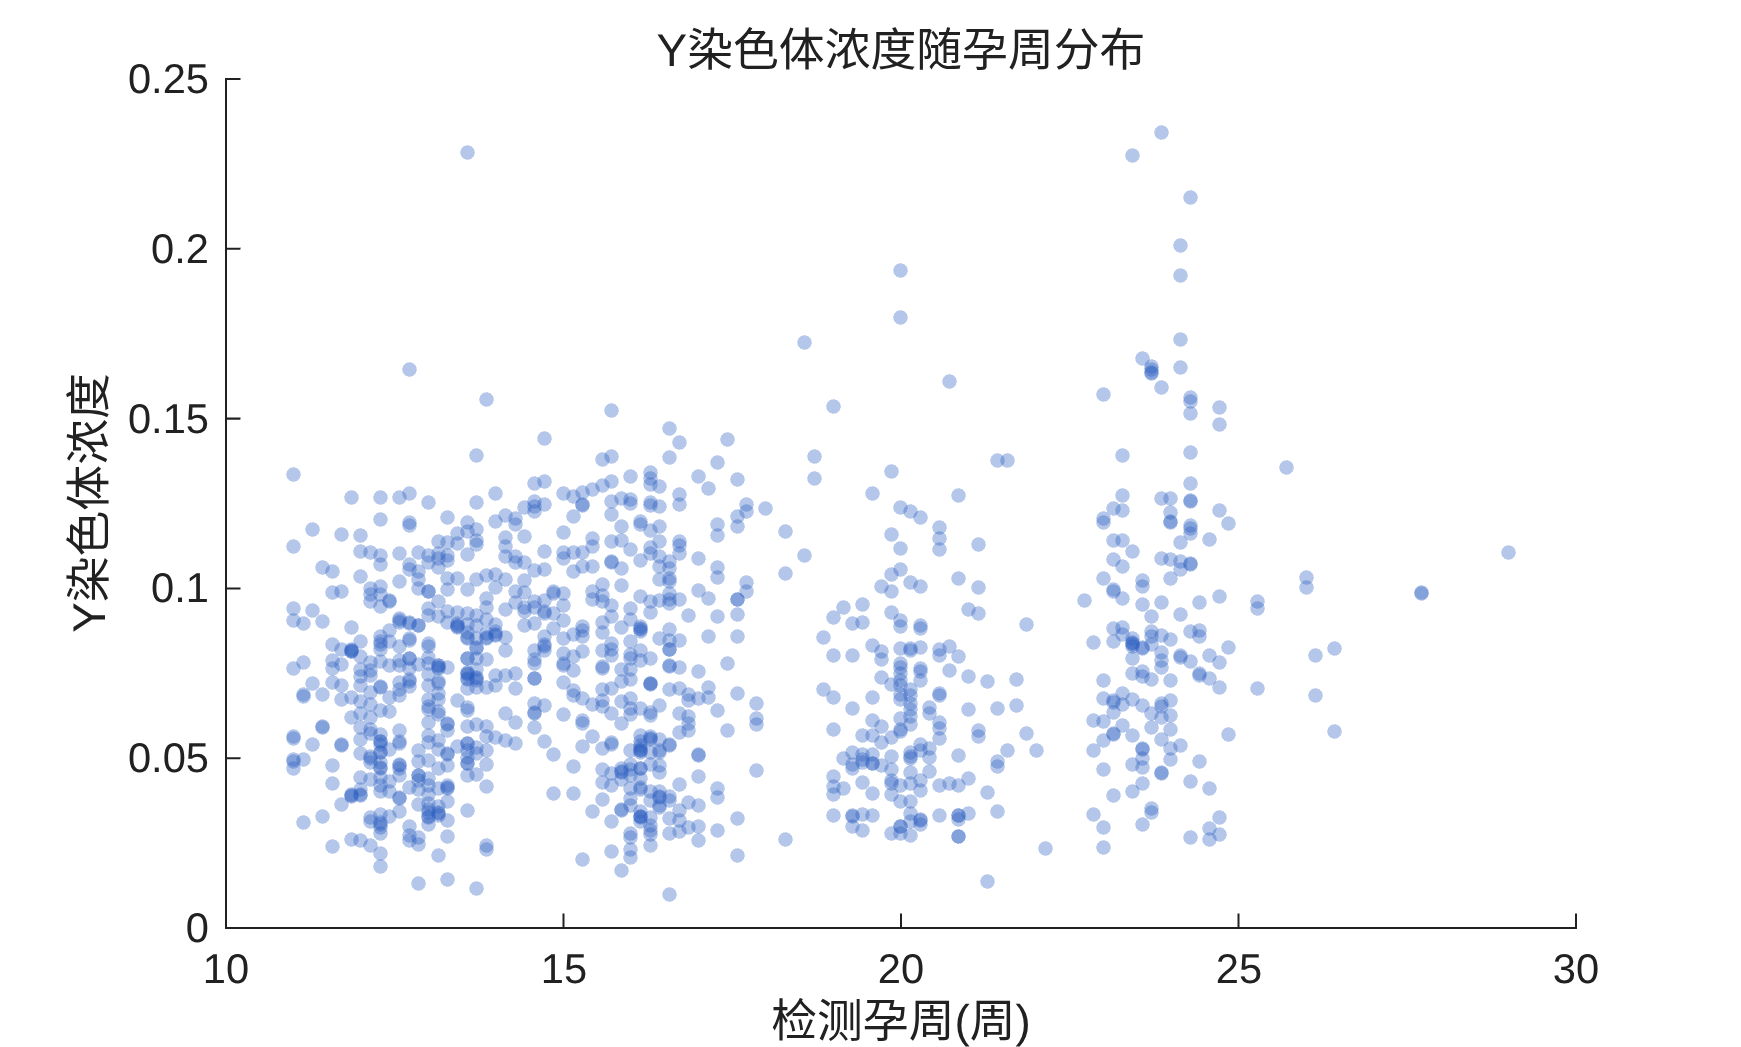
\includegraphics[width=0.48\textwidth]{q1_scatter_gest.png}
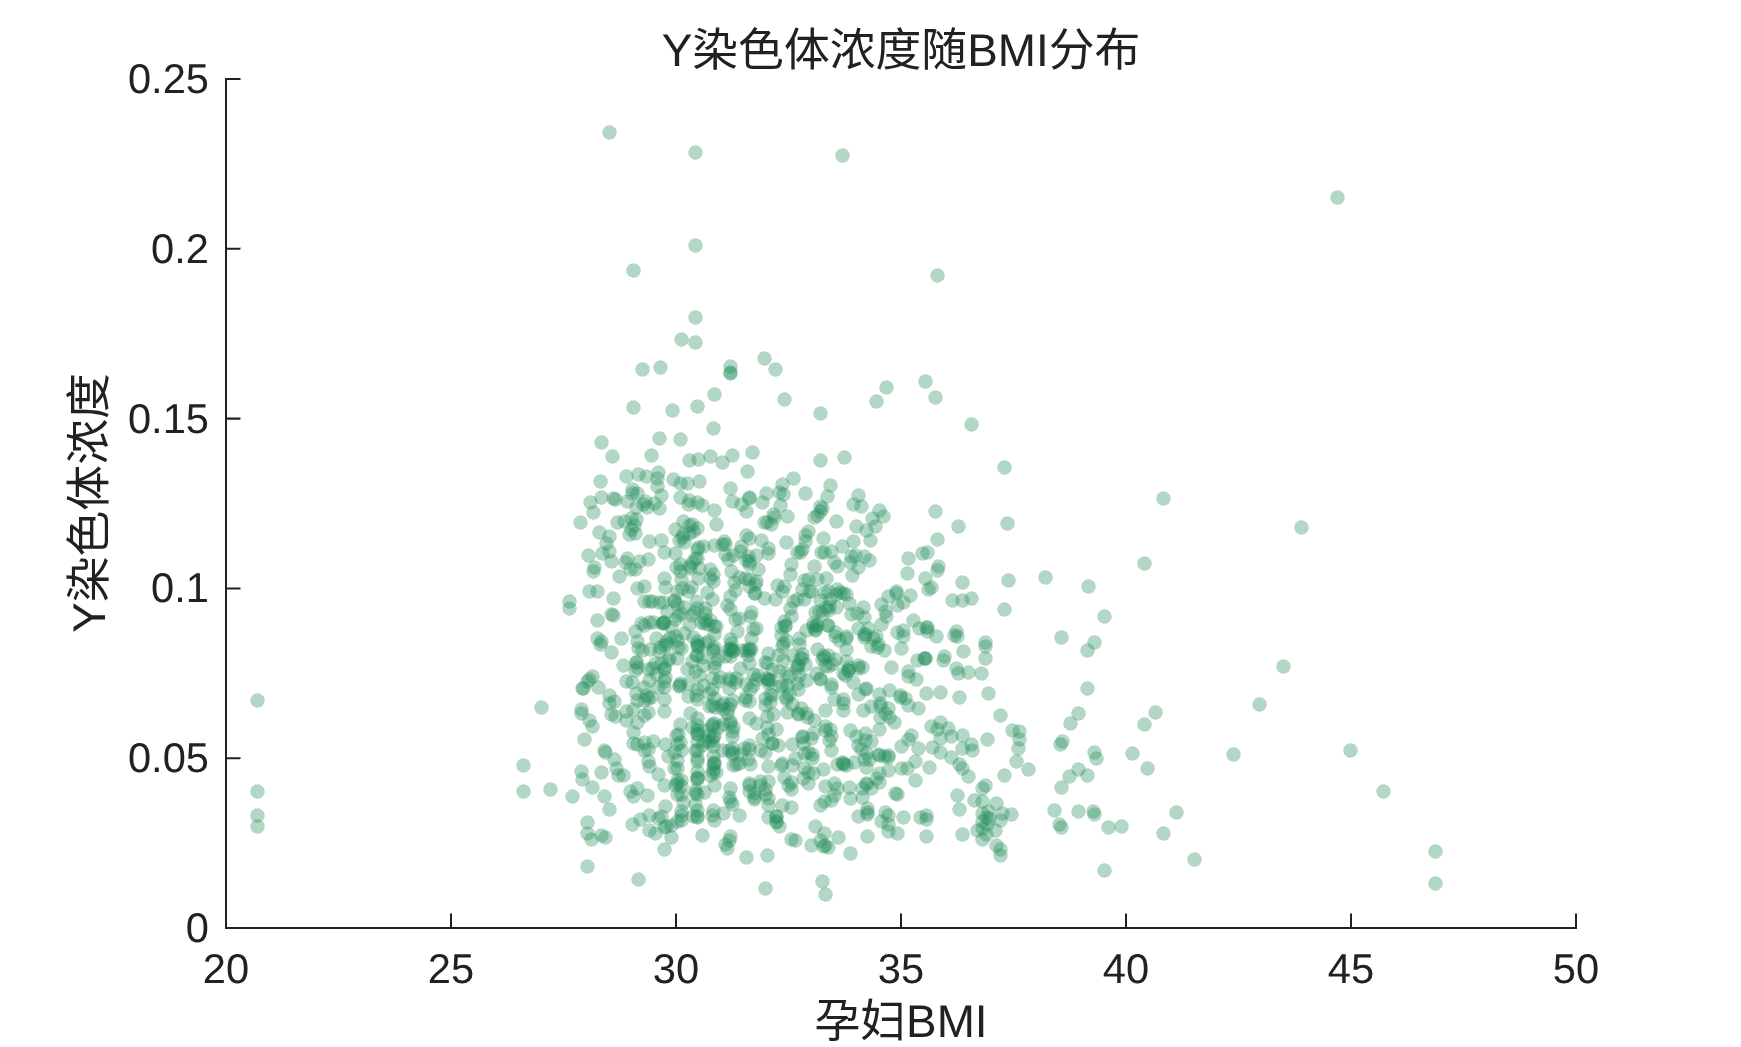
\includegraphics[width=0.48\textwidth]{q1_scatter_bmi.png}
\caption{Y 染色体浓度与孕周、BMI 的散点关系}
\label{fig:q1scatter}
\end{figure}

为同时观察变量之间的线性相关结构，图 \ref{fig:q1heatmap} 给出相关性热力图。孕周、BMI、年龄和体重与 Y 染色体浓度的方向与表 \ref{tab:q1corr} 一致。GC 含量相关性不显著，过滤比例虽达到 0.05 水平附近，但相关系数绝对值较小。

\begin{figure}[H]
\centering
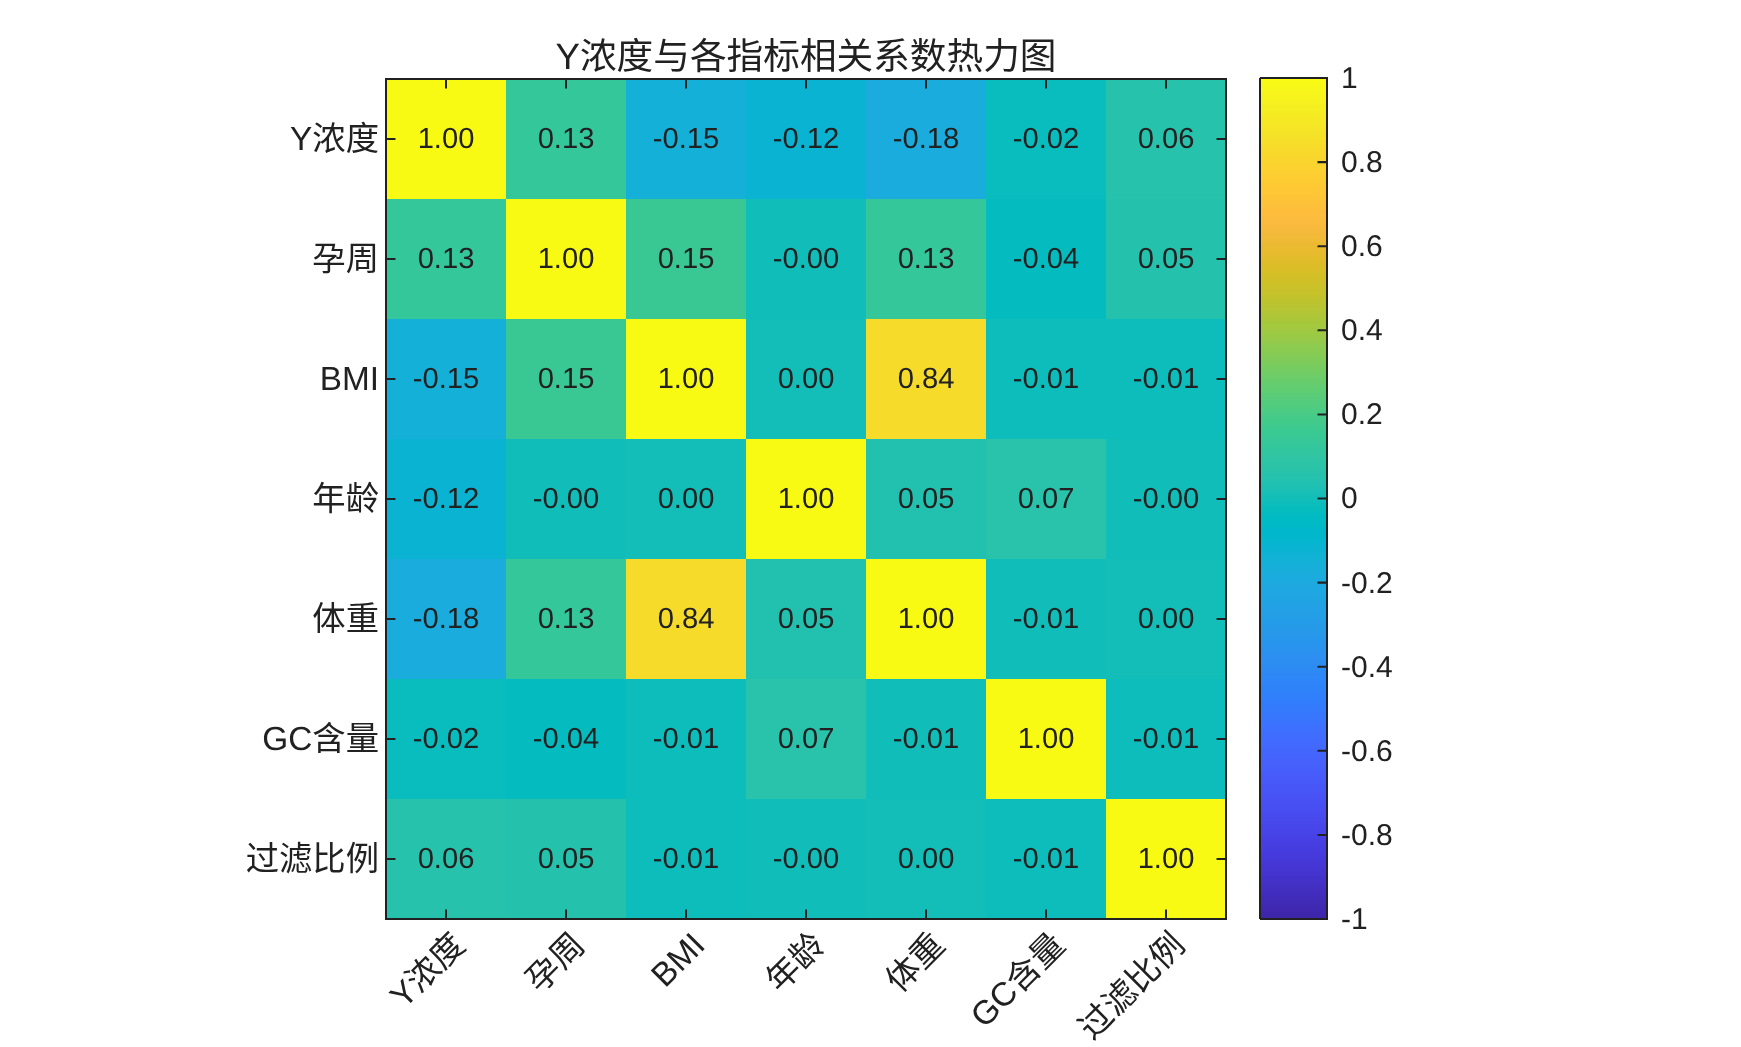
\includegraphics[width=0.72\textwidth]{q1_corr_heatmap.png}
\caption{主要变量相关性热力图}
\label{fig:q1heatmap}
\end{figure}

\subsection{回归模型建立}

在相关性分析基础上，建立基础多元线性回归模型：
\begin{equation}
Y_i=\beta_0+\beta_1t_i+\beta_2B_i+\beta_3Age_i+\beta_4GC_i+\beta_5Filter_i+\varepsilon_i.
\end{equation}
其中 $Filter_i$ 表示被过滤掉读段数的比例。BMI 已综合反映身高和体重形成的体型差异，因此主模型不同时放入 BMI、身高和体重。为检验孕周与 BMI 是否存在交互影响，进一步建立交互项模型：
\begin{equation}
Y_i=\beta_0+\beta_1t_i+\beta_2B_i+\beta_3t_iB_i+\beta_4Age_i+\beta_5GC_i+\beta_6Filter_i+\varepsilon_i.
\end{equation}
同时建立二次模型和身高体重对照模型，用于比较拟合效果。参数采用普通最小二乘估计：
\begin{equation}
\hat{\bm{\beta}}=(\bm{X}^{\mathsf T}\bm{X})^{-1}\bm{X}^{\mathsf T}\bm{Y}.
\end{equation}

\subsection{模型求解与显著性检验}

表 \ref{tab:q1goodness} 给出四类回归模型的拟合优度。交互项模型的调整 $R^2$ 为 0.0583，略高于基础模型，且整体 F 检验显著，因此本文选择交互项模型作为问题一主模型，并取其残差标准差 $\sigma=0.0325$ 作为后续误差参数。

\begin{table}[H]
\centering
\caption{问题一回归模型拟合优度}
\label{tab:q1goodness}
\begin{tabular}{lrrrrr}
\toprule
模型 & $R^2$ & 调整 $R^2$ & F 值 & F 检验 $p$ 值 & 残差标准差 \\
\midrule
基础模型 & 0.0625 & 0.0581 & 14.3349 & $1.31\times10^{-13}$ & 0.0325 \\
交互项模型 & 0.0636 & 0.0583 & 12.1599 & $2.91\times10^{-13}$ & 0.0325 \\
二次模型 & 0.0565 & 0.0521 & 12.8782 & $3.48\times10^{-12}$ & 0.0326 \\
身高体重对照 & 0.0712 & 0.0660 & 13.7310 & $4.44\times10^{-15}$ & 0.0324 \\
\bottomrule
\end{tabular}
\end{table}

交互项模型的关键系数见表 \ref{tab:q1reg}. BMI 系数为 $-0.00351$，在 0.05 水平下显著，表明在控制其他因素后 BMI 越高，Y 染色体浓度越低。年龄系数同样为负且显著。交互项 $t\times BMI$ 的 $p$ 值为 0.2605，未达到显著水平，但模型调整 $R^2$ 略有提升，且该项对后续分组时点预测具有解释上的连续性，因此在主模型中保留。

\begin{table}[H]
\centering
\caption{问题一交互项模型主要回归结果}
\label{tab:q1reg}
\begin{tabular}{lrrrr}
\toprule
变量 & 系数 & 标准误 & $t$ 值 & $p$ 值 \\
\midrule
截距 & 0.21737 & 0.12817 & 1.696 & 0.0902 \\
孕周 & -0.00163 & 0.00256 & -0.640 & 0.5226 \\
BMI & -0.00351 & 0.00143 & -2.463 & 0.0139 \\
$t\times BMI$ & $8.82\times10^{-5}$ & $7.84\times10^{-5}$ & 1.126 & 0.2605 \\
年龄 & -0.00108 & 0.00027 & -3.972 & $7.61\times10^{-5}$ \\
GC 含量 & -0.06978 & 0.30001 & -0.233 & 0.8161 \\
过滤比例 & 0.51056 & 0.29112 & 1.754 & 0.0798 \\
\bottomrule
\end{tabular}
\end{table}

图 \ref{fig:q1resid} 展示主模型残差与拟合值的关系。残差围绕 0 分布，但离散程度较明显，与较低 $R^2$ 的结果一致。这说明模型能够捕捉 Y 浓度与孕周、BMI 等因素之间的统计趋势，但个体层面的随机波动仍不可忽视。后续问题二、三不直接把该回归解释为精确个体预测，而是用于估计组内达标比例和误差影响。

\begin{figure}[H]
\centering
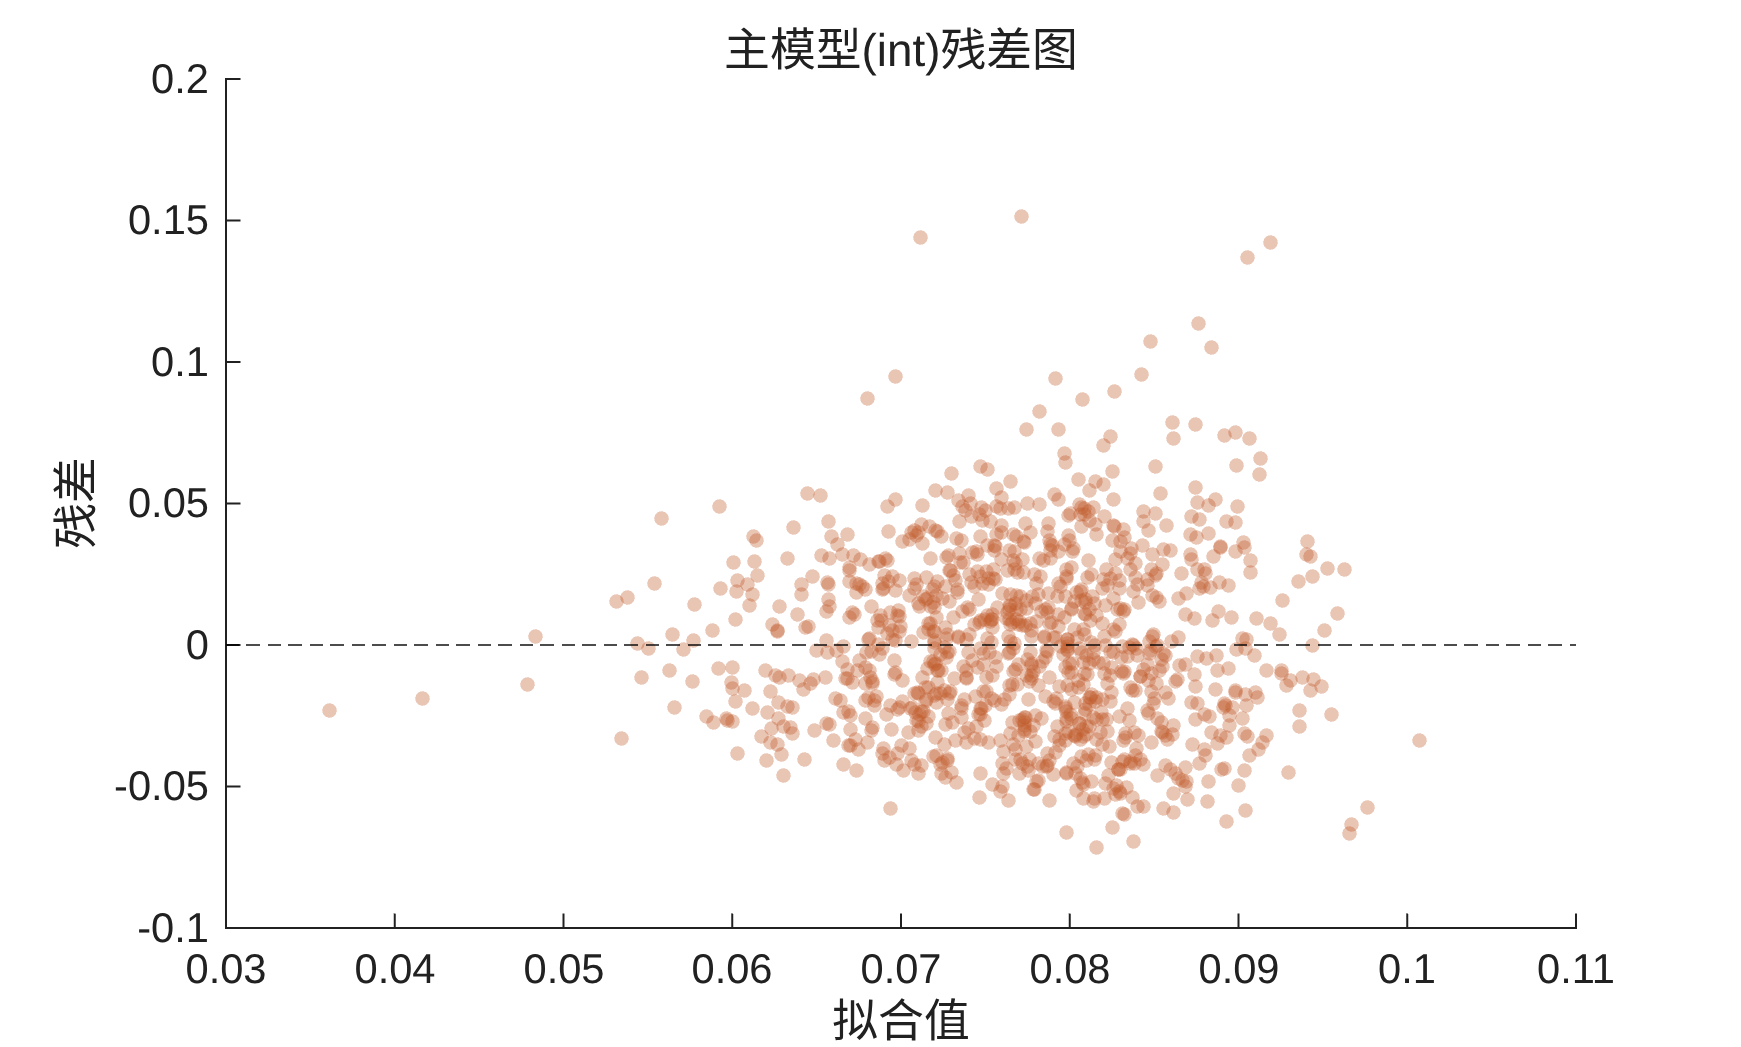
\includegraphics[width=0.68\textwidth]{q1_resid.png}
\caption{问题一主模型残差图}
\label{fig:q1resid}
\end{figure}

此外，剔除男胎 AB 列非空记录后重新估计基础模型，孕周系数由 0.00123 变为 0.00148，BMI 系数由 -0.00195 变为 -0.00200，方向保持一致。该对比说明，保留男胎 AB 非空记录未改变问题一核心变量的方向性结论。

\section{问题二：基于 BMI 分组的最佳 NIPT 时点选择}

\subsection{达标比例模型}

问题二只以 BMI 为主要影响因素。本文使用男胎全部 1082 条记录估计简化回归模型：
\begin{equation}
\hat{Y}_i(t,B_i)=\alpha_0+\alpha_1t+\alpha_2B_i+\alpha_3tB_i.
\end{equation}
对第 $i$ 名孕妇，使用其平均 BMI $\bar{B}_i$ 代入模型。给定 BMI 分组 $G_g$ 和检测时点 $t$，组内预测达标比例定义为
\begin{equation}
p_g(t)=\frac{1}{N_g}\sum_{i\in G_g}\mathbf{1}\left(\hat{Y}_i(t,\bar{B}_i)\ge 0.04\right).
\end{equation}
该定义以孕妇为计数单位，同一孕妇的多次检测记录不会在分组优化中重复计权。

\subsection{风险函数与切点搜索}

为刻画检测时点的临床代价，定义分段时间风险：
\begin{equation}
C(t)=
\begin{cases}
1,&t<13,\\
5,&13\le t<28,\\
20,&t\ge 28.
\end{cases}
\end{equation}
第 $g$ 组在时点 $t$ 的总风险为
\begin{equation}
R_g(t)=C(t)+\lambda[1-p_g(t)],
\end{equation}
其中 $\lambda$ 为不达标惩罚系数，基准值取 $\lambda=10$。

将 267 名男胎孕妇按平均 BMI 升序排列，设切点为 $c_1,c_2,c_3$，形成 $K=4$ 个连续 BMI 区间。优化目标为
\begin{equation}
\min_{c_1,c_2,c_3}\sum_{g=1}^{4}\min_{t\in T}R_g(t),
\end{equation}
其中候选时点集合为
\begin{equation}
T=\left\{10,10+\frac{1}{7},10+\frac{2}{7},\ldots,25\right\}.
\end{equation}
约束条件为每组孕妇数 $N_g\ge 20$，且 BMI 区间连续、无重叠。

\subsection{分组和推荐时点结果}

图 \ref{fig:q2bmi} 给出了男胎孕妇平均 BMI 的分布及最优切点位置。前三个分组样本数均为 20，高 BMI 组样本数为 207，说明样本 BMI 分布右侧较集中。由于前三个低 BMI 小组在风险函数下均达到最早时点最优，边界值 28.89、29.52、30.05 的临床区分度不宜过度解释。

\begin{figure}[H]
\centering
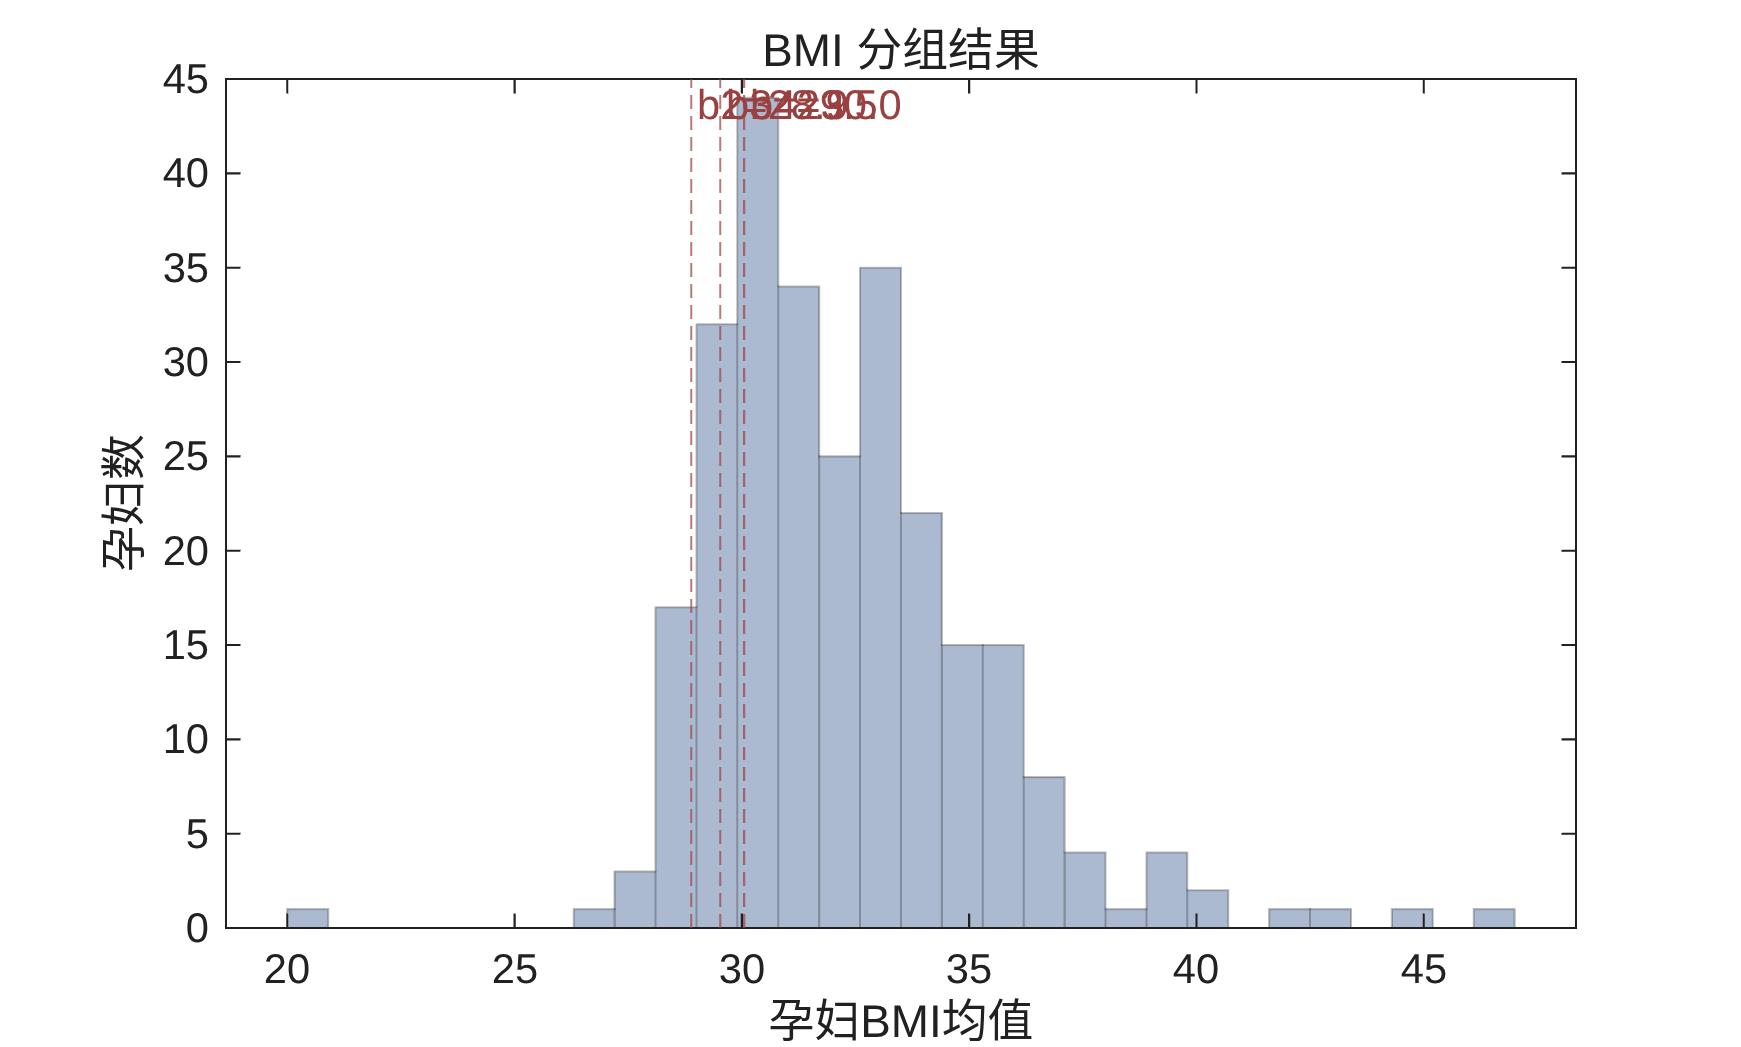
\includegraphics[width=0.72\textwidth]{q2_bmi_groups.png}
\caption{问题二 BMI 分组结果}
\label{fig:q2bmi}
\end{figure}

表 \ref{tab:q2result} 给出问题二分组与最佳检测时点。低 BMI 三组推荐时点均为 10 周，高 BMI 组推荐时点为 12.29 周，约为 12 周 2 天。若用于简化临床表述，可将前三组概括为 BMI 不超过 30.05 的孕妇建议 10 周检测，BMI 高于 30.05 的孕妇建议约 12.3 周检测。

\begin{table}[H]
\centering
\caption{问题二 BMI 分组与最佳 NIPT 时点}
\label{tab:q2result}
\begin{tabular}{clrrrr}
\toprule
组别 & BMI 区间 & 孕妇数 & 最佳时点/周 & 达标比例 & 总风险 \\
\midrule
1 & $[20.70,28.89)$ & 20 & 10.00 & 1.000 & 1.000 \\
2 & $[28.89,29.52)$ & 20 & 10.00 & 1.000 & 1.000 \\
3 & $[29.52,30.05)$ & 20 & 10.00 & 1.000 & 1.000 \\
4 & $[30.05,46.88)$ & 207 & 12.29 & 0.995 & 1.048 \\
\bottomrule
\end{tabular}
\end{table}

图 \ref{fig:q2curve} 展示各组达标比例和总风险随检测时点的变化。低 BMI 组在 10 周已能达到较高达标比例，因此更早检测具有更低时间风险；高 BMI 组需要略推迟至 12.29 周，以降低不达标惩罚。

\begin{figure}[H]
\centering
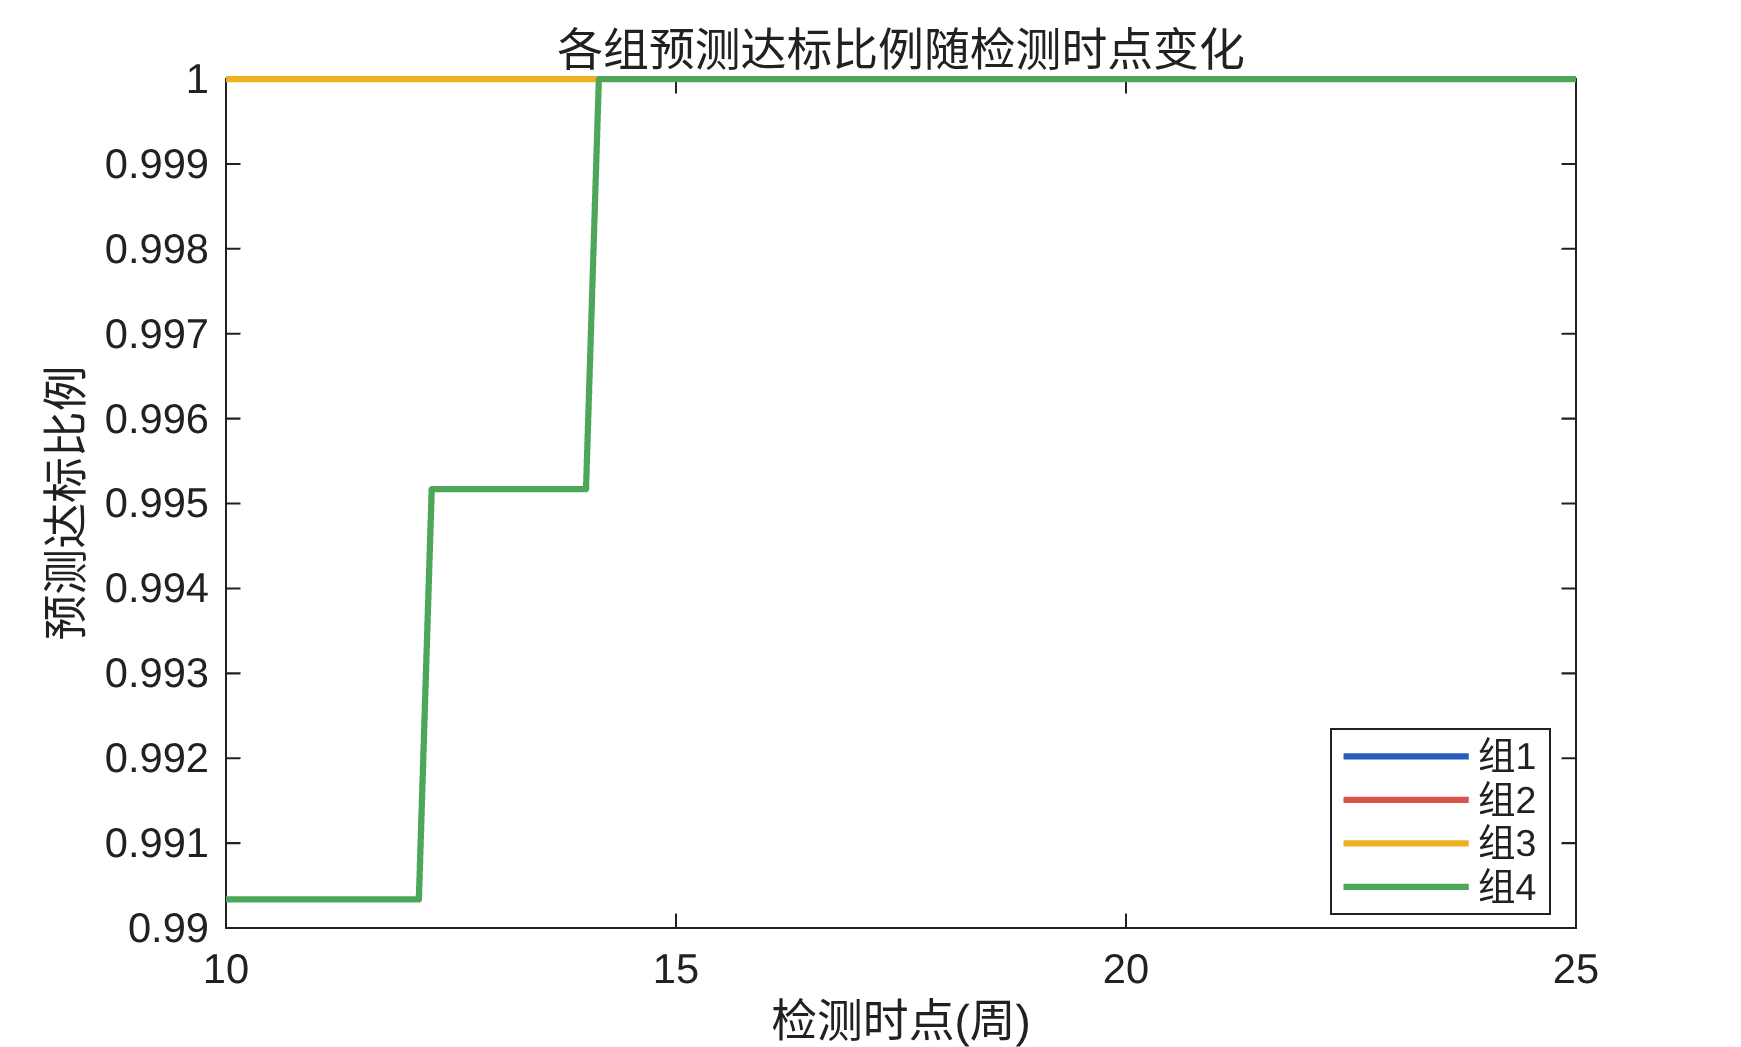
\includegraphics[width=0.48\textwidth]{q2_p_reach_curves.png}
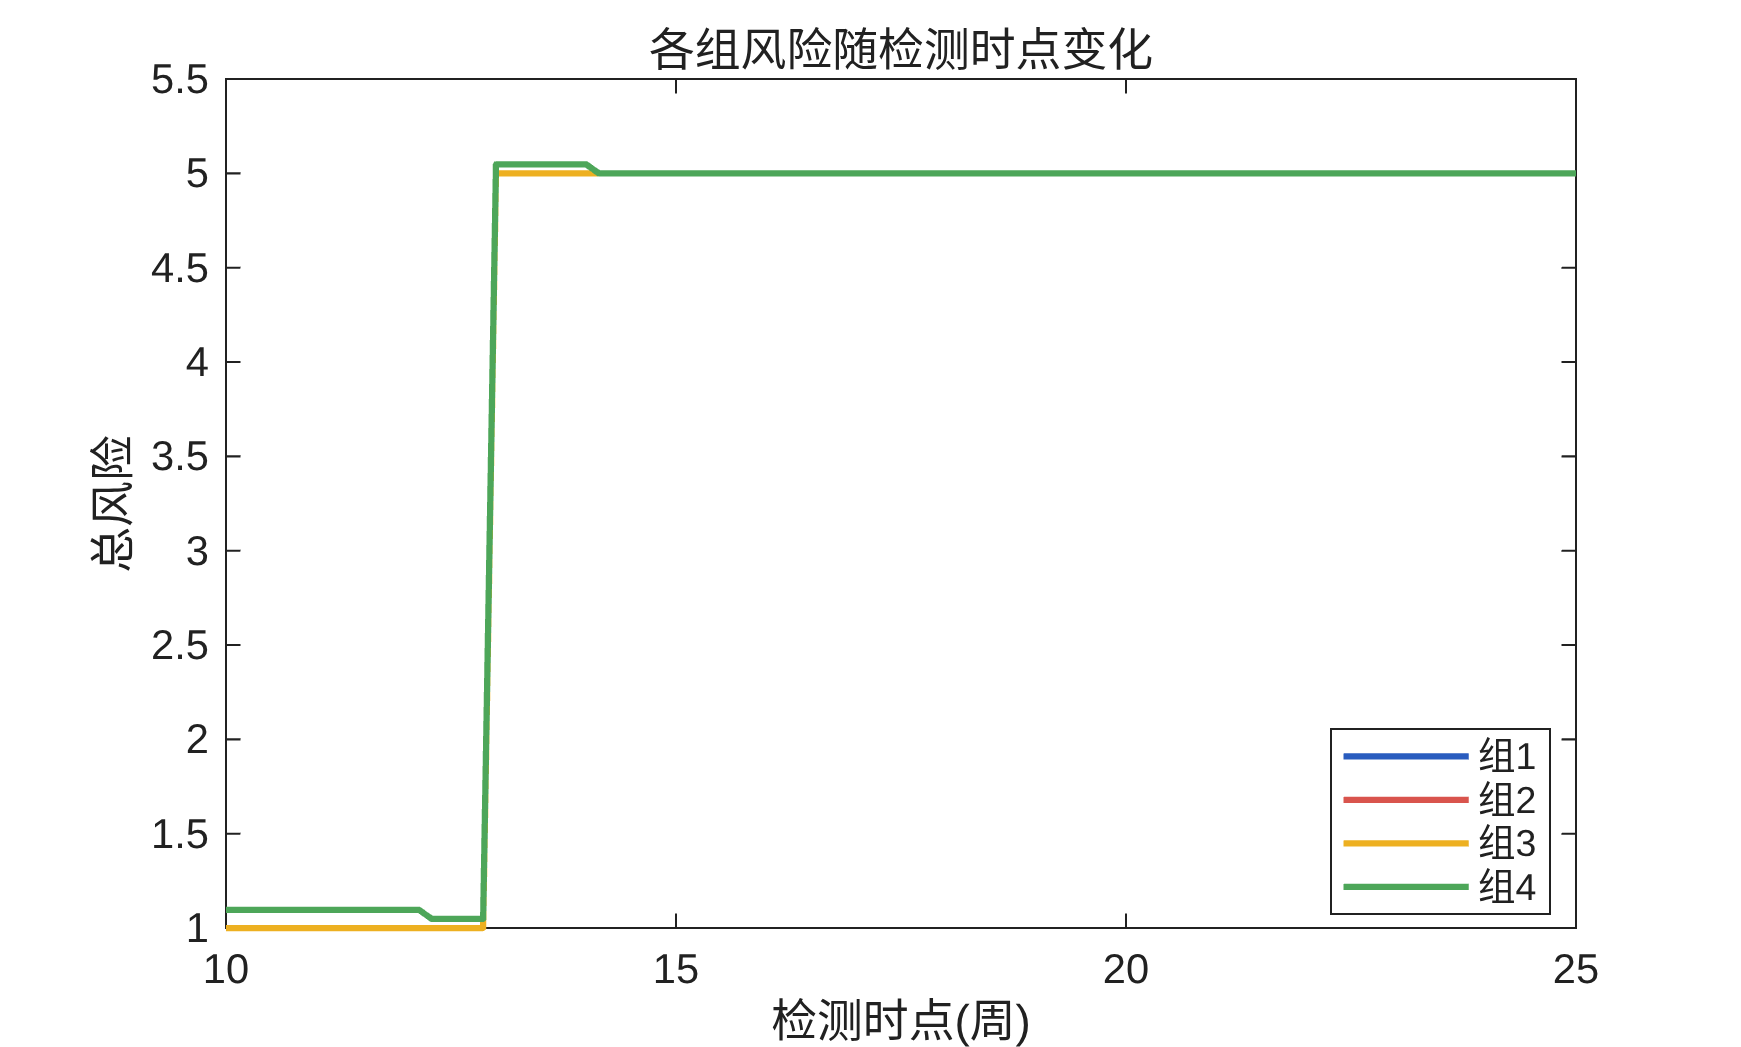
\includegraphics[width=0.48\textwidth]{q2_risk_curves.png}
\caption{问题二各 BMI 组达标比例和总风险曲线}
\label{fig:q2curve}
\end{figure}

\subsection{检测误差影响分析}

以问题一主模型残差标准差 $\sigma=0.0325$ 作为检测误差尺度，进行 500 次蒙特卡洛扰动。扰动过程中固定回归系数和 BMI 切点，只对预测浓度加入正态误差：
\begin{equation}
\hat{Y}_i^{(m)}(t)=\hat{Y}_i(t)+e_i^{(m)},\qquad e_i^{(m)}\sim N(0,\sigma^2).
\end{equation}
表 \ref{tab:q2mc} 给出扰动后的推荐时点分布。前三组均值约为 10.4 至 10.5 周，高 BMI 组均值为 12.47 周。扰动范围未超过 12.86 周，说明问题二推荐时点对检测误差具有一定稳定性。

\begin{table}[H]
\centering
\caption{问题二检测误差蒙特卡洛分析}
\label{tab:q2mc}
\begin{tabular}{crrrr}
\toprule
组别 & 时点均值/周 & 标准差/周 & 最小值/周 & 最大值/周 \\
\midrule
1 & 10.43 & 0.83 & 10.00 & 12.86 \\
2 & 10.41 & 0.79 & 10.00 & 12.86 \\
3 & 10.50 & 0.86 & 10.00 & 12.86 \\
4 & 12.47 & 0.41 & 10.29 & 12.86 \\
\bottomrule
\end{tabular}
\end{table}

进一步改变 $\lambda$ 进行灵敏度分析。当 $\lambda$ 分别取 5、10、20 时，四组推荐时点仍为 10、10、10、12.29 周，BMI 边界保持 $20.70,28.89,29.52,30.05,46.88$。这表明在问题二的简化模型下，不达标惩罚权重变化未改变分组和推荐时点。

\section{问题三：多因素修正下的分组与时点优化}

\subsection{测序质量综合指标}

问题三需要综合检测误差和多种协变量。本文将原始读段数、比对比例、重复读段比例、唯一比对读段数、过滤比例和 GC 中心偏离构造成测序质量指标。对一般变量采用 Z-score 标准化：
\begin{equation}
Z_{ik}=\frac{X_{ik}-\bar{X}_k}{s_k}.
\end{equation}
为统一方向，定义
\begin{equation}
q_L=Z_L,\quad q_M=Z_M,\quad q_N=-Z_N,\quad q_O=Z_O,\quad q_{AA}=-Z_{AA},
\end{equation}
其中 $L$ 为原始读段数，$M$ 为比对比例，$N$ 为重复读段比例，$O$ 为唯一比对读段数，$AA$ 为过滤比例。GC 含量按中心偏离处理：
\begin{equation}
q_{GC}=-\frac{|GC_i-\overline{GC}|}{s_{GC}}.
\end{equation}
等权质量指标为
\begin{equation}
Q_i=\frac{1}{6}(q_L+q_M+q_N+q_O+q_{AA}+q_{GC}).
\end{equation}
PCA 权重作为对比方案\cite{jolliffe2002}。表 \ref{tab:q3weight} 显示，PCA 权重主要集中在原始读段数和唯一比对读段数上；等权和 PCA 权重得到的推荐时点一致，因此正文采用等权指标作为主结果。

\begin{table}[H]
\centering
\caption{问题三测序质量指标权重}
\label{tab:q3weight}
\begin{tabular}{lrr}
\toprule
指标 & 等权权重 & PCA 权重 \\
\midrule
原始读段数 & 0.1667 & 0.3755 \\
比对比例 & 0.1667 & 0.0601 \\
重复读段比例（取反） & 0.1667 & 0.0207 \\
唯一比对读段数 & 0.1667 & 0.3705 \\
过滤比例（取反） & 0.1667 & 0.1590 \\
GC 中心偏离（取反） & 0.1667 & 0.0142 \\
\bottomrule
\end{tabular}
\end{table}

\subsection{多因素回归与达标概率}

以记录层男胎数据估计多因素回归模型：
\begin{equation}
\hat{Y}_i=\gamma_0+\gamma_1t_i+\gamma_2B_i+\gamma_3Age_i+\gamma_4G_i+\gamma_5P_i
+\gamma_6IUI_i+\gamma_7IVF_i+\gamma_8Q_i+\gamma_9t_iB_i.
\end{equation}
其中 $G_i$ 为怀孕次数，$P_i$ 为生产次数，$IUI_i$ 和 $IVF_i$ 为妊娠方式哑变量，自然受孕为基准组。表 \ref{tab:q3reg} 给出主模型关键结果。年龄、BMI 和质量指标 $Q$ 的影响在统计上显著；孕周主效应和 $t\times BMI$ 交互项未达到显著水平，但保留在模型中以保持时点预测结构。

\begin{table}[H]
\centering
\caption{问题三多因素回归主模型结果}
\label{tab:q3reg}
\begin{tabular}{lrrrr}
\toprule
变量 & 系数 & 标准误 & $t$ 值 & $p$ 值 \\
\midrule
截距 & 0.18494 & 0.04615 & 4.008 & $6.56\times10^{-5}$ \\
孕周 & -0.00079 & 0.00252 & -0.314 & 0.7533 \\
BMI & -0.00297 & 0.00141 & -2.103 & 0.0357 \\
年龄 & -0.00112 & 0.00028 & -4.046 & $5.57\times10^{-5}$ \\
怀孕次数 & -0.00010 & 0.00149 & -0.067 & 0.9465 \\
生产次数 & 0.00204 & 0.00197 & 1.033 & 0.3018 \\
IUI & 0.01556 & 0.01088 & 1.430 & 0.1531 \\
IVF & -0.01595 & 0.01165 & -1.370 & 0.1711 \\
质量指标 $Q$ & -0.01154 & 0.00220 & -5.248 & $1.86\times10^{-7}$ \\
$t\times BMI$ & $5.83\times10^{-5}$ & $7.74\times10^{-5}$ & 0.752 & 0.4521 \\
\bottomrule
\end{tabular}
\end{table}

将回归模型转化到孕妇层面时，BMI 和质量指标采用该孕妇历次检测均值，年龄、孕情和妊娠方式取其固定值。设预测浓度为 $\hat{Y}_i(t)$，检测误差标准差为 $\sigma$，则第 $i$ 名孕妇在孕周 $t$ 检测时达标的概率定义为
\begin{equation}
\pi_i(t)=\Phi\left(\frac{\hat{Y}_i(t)-0.04}{\sigma}\right),
\end{equation}
其中 $\Phi(\cdot)$ 为标准正态分布函数。第 $g$ 组的平均达标比例为
\begin{equation}
p_g(t)=\frac{1}{N_g}\sum_{i\in G_g}\pi_i(t).
\end{equation}

\subsection{带达标约束的时点优化}

问题三沿用问题二的时间风险和不达标惩罚，并增加达标比例约束：
\begin{equation}
\min \sum_{g=1}^{4}R_g(t_g),\qquad
R_g(t_g)=C(t_g)+\lambda[1-p_g(t_g)],
\end{equation}
\begin{equation}
p_g(t_g)\ge \eta,\quad N_g\ge 20,\quad t_g\in T.
\end{equation}
本文基准取 $\eta=0.85$。若某组在 $T$ 内不能满足该约束，则取 $p_g(t)$ 最大的时点，并在结果中标注。实际求解中四组均满足 $\eta=0.85$，但高 BMI 组的最优时点达到候选上界 25 周，需要在解释中保留这一限制。

表 \ref{tab:q3result} 给出问题三分组和推荐时点。与问题二相比，前三组推荐时点均从 10 周后移至 12.86 周；第四组从 12.29 周后移至 25 周。图 \ref{fig:q3compare} 直观展示了这种变化。

\begin{table}[H]
\centering
\caption{问题三多因素修正后的 BMI 分组与推荐时点}
\label{tab:q3result}
\begin{tabular}{clrrrr}
\toprule
组别 & BMI 区间 & 孕妇数 & 推荐时点/周 & 达标比例 & 总风险 \\
\midrule
1 & $[20.70,28.89)$ & 20 & 12.86 & 0.897 & 2.032 \\
2 & $[28.89,29.52)$ & 20 & 12.86 & 0.887 & 2.126 \\
3 & $[29.52,30.10)$ & 22 & 12.86 & 0.879 & 2.209 \\
4 & $[30.10,46.88)$ & 205 & 25.00 & 0.908 & 5.917 \\
\bottomrule
\end{tabular}
\end{table}

\begin{figure}[H]
\centering
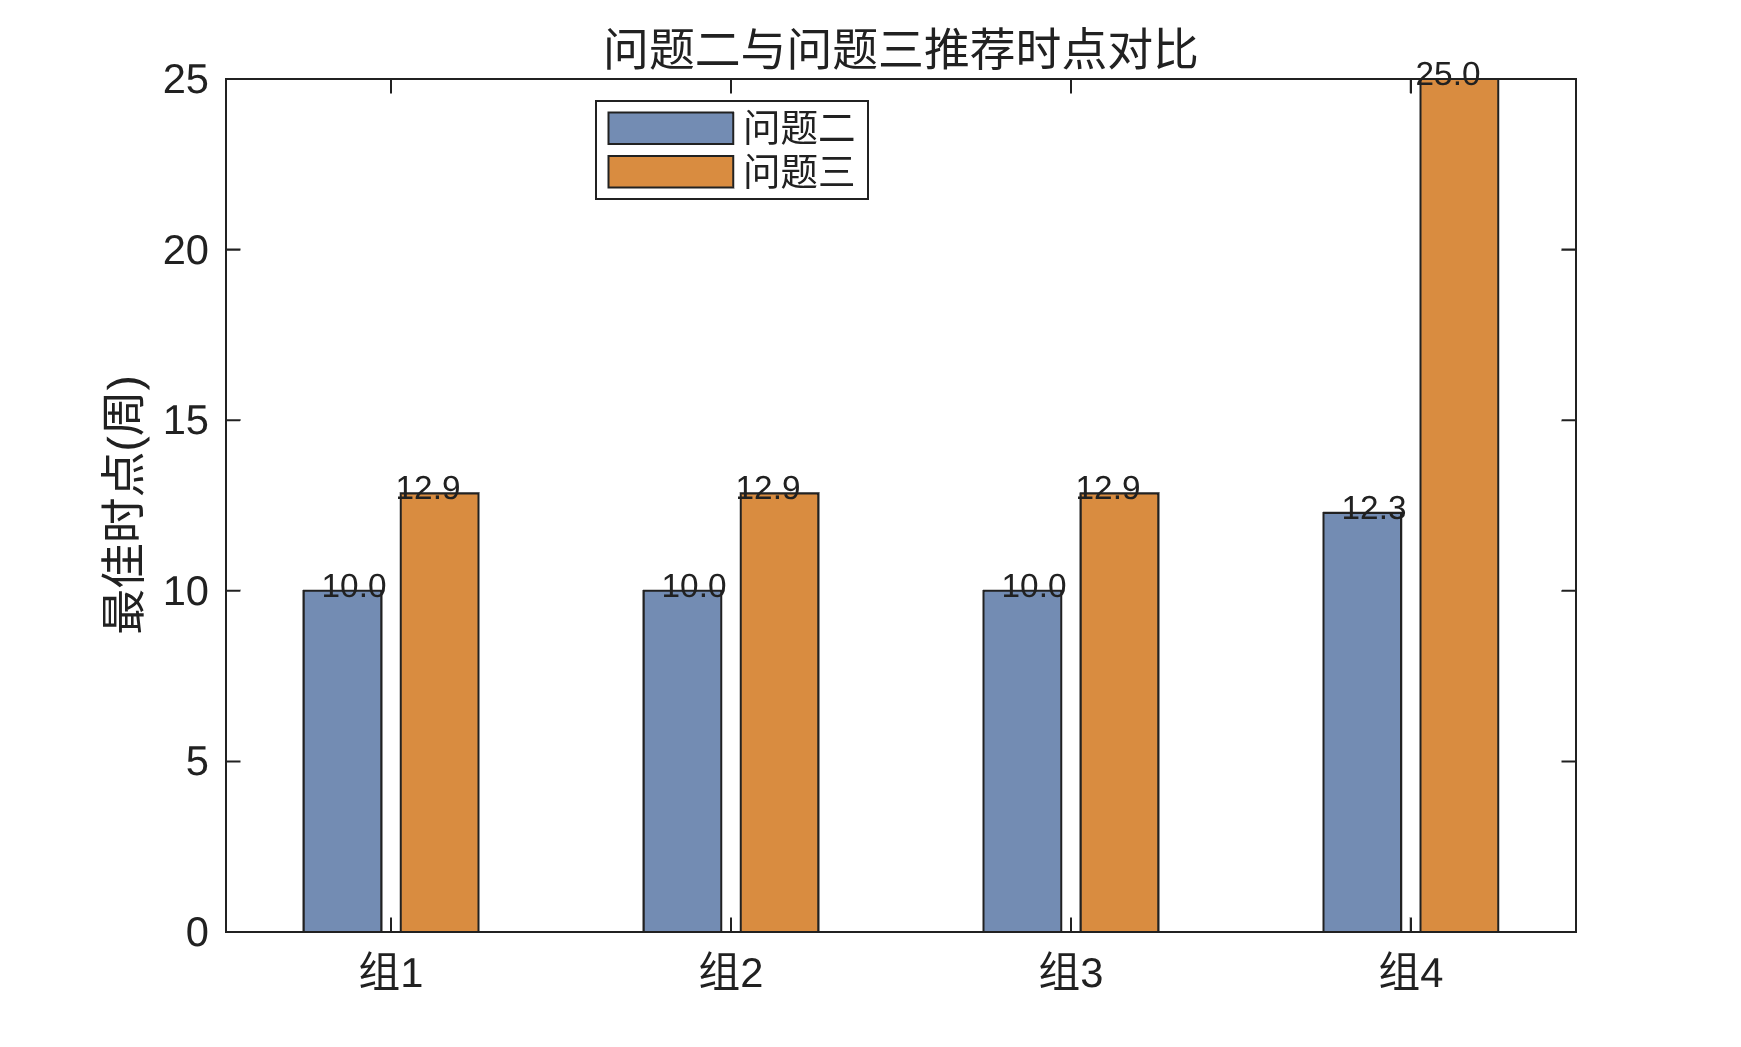
\includegraphics[width=0.72\textwidth]{q3_compare_q2.png}
\caption{问题二与问题三推荐时点对比}
\label{fig:q3compare}
\end{figure}

多因素重要性见图 \ref{fig:q3importance}。标准化系数显示，年龄、质量指标 $Q$ 和 BMI 对 Y 浓度预测的影响较突出。质量指标 $Q$ 的回归系数为负，说明在当前数据和质量指标构造下，测序质量变量与浓度观测之间存在复杂关系；该结果不应解释为“质量越高浓度越低”的因果结论，而应作为误差修正项进入达标概率估计。

\begin{figure}[H]
\centering
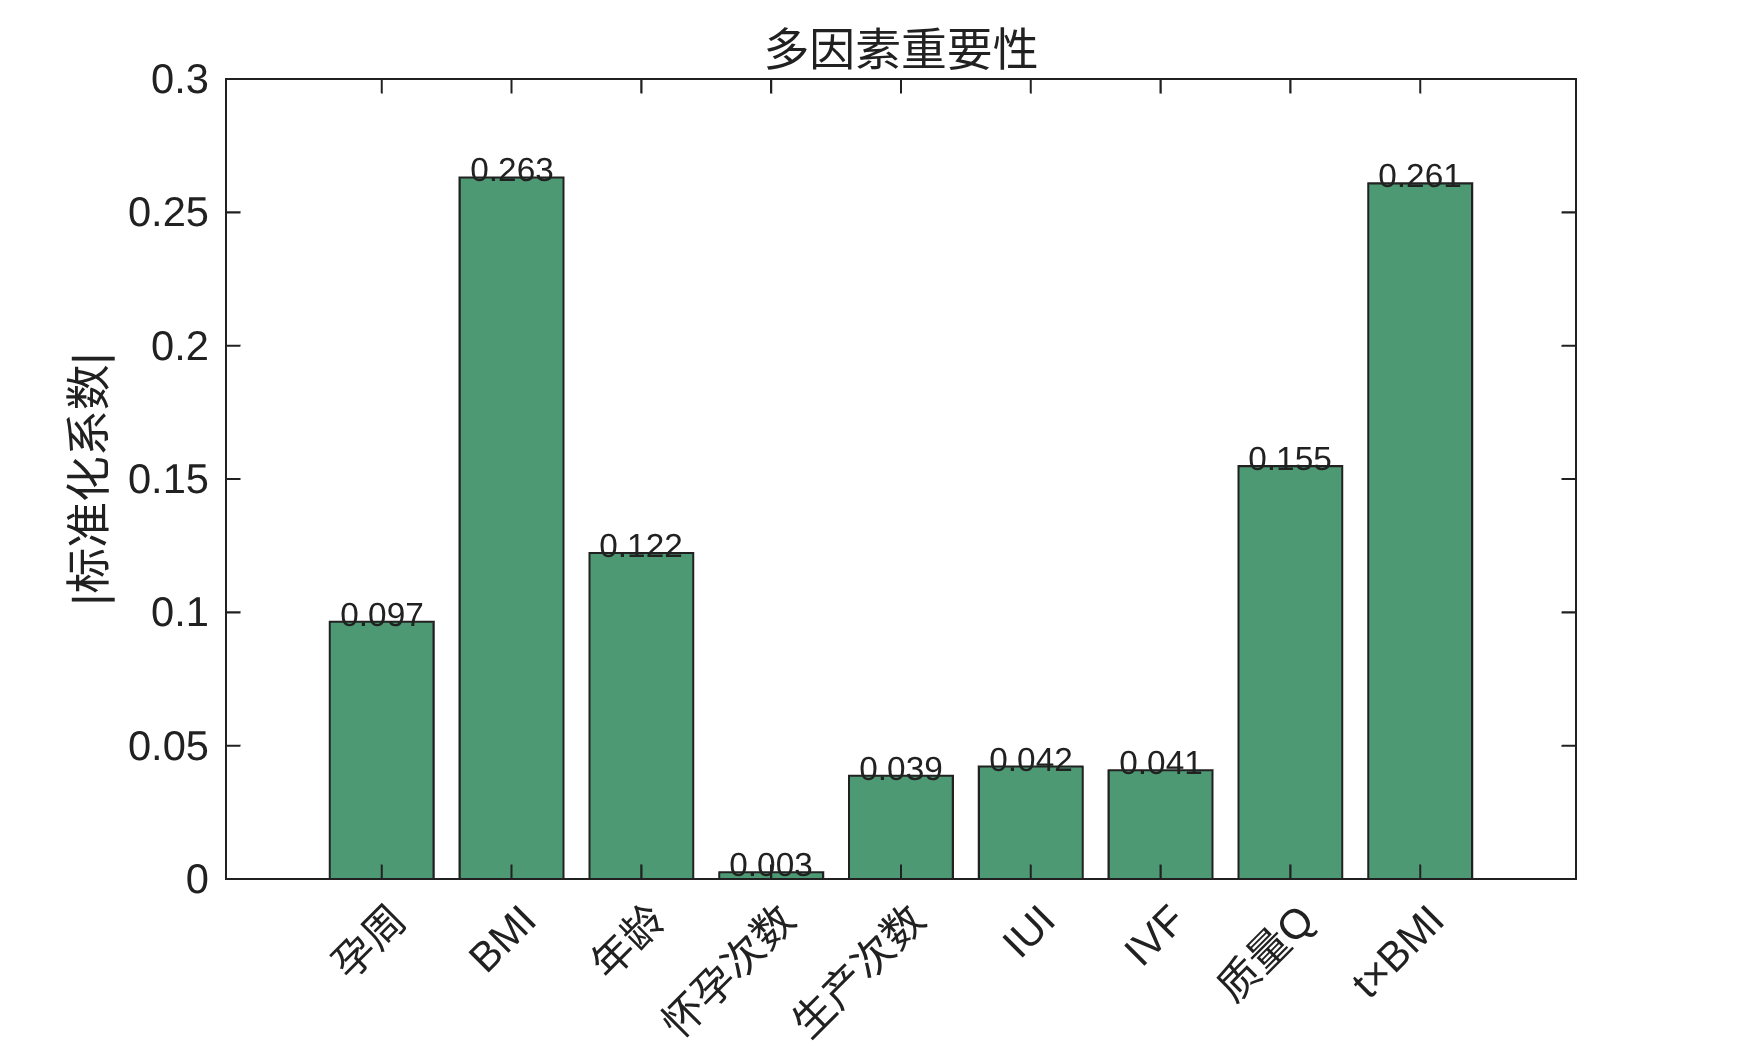
\includegraphics[width=0.72\textwidth]{q3_importance.png}
\caption{问题三多因素重要性}
\label{fig:q3importance}
\end{figure}

\subsection{灵敏度分析}

为检验可靠性约束对问题三结果的影响，改变 $\eta$ 并固定问题三主分组，结果见表 \ref{tab:senseta}. 当 $\eta=0.80$ 时，四组均可在 12.86 周满足约束；当 $\eta=0.85$ 时，高 BMI 组需推迟至 25 周；当 $\eta=0.90$ 时，四组均推迟至 25 周；当 $\eta=0.95$ 时，四组在 25 周内均未达到约束。图 \ref{fig:senseta} 展示了该变化过程。

\begin{table}[H]
\centering
\caption{不同达标比例约束下的问题三推荐时点}
\label{tab:senseta}
\begin{tabular}{crrrrr}
\toprule
$\eta$ & 组1/周 & 组2/周 & 组3/周 & 组4/周 & 是否全部满足约束 \\
\midrule
0.80 & 12.86 & 12.86 & 12.86 & 12.86 & 是 \\
0.85 & 12.86 & 12.86 & 12.86 & 25.00 & 是 \\
0.90 & 25.00 & 25.00 & 25.00 & 25.00 & 是 \\
0.95 & 25.00 & 25.00 & 25.00 & 25.00 & 否 \\
\bottomrule
\end{tabular}
\end{table}

\begin{figure}[H]
\centering
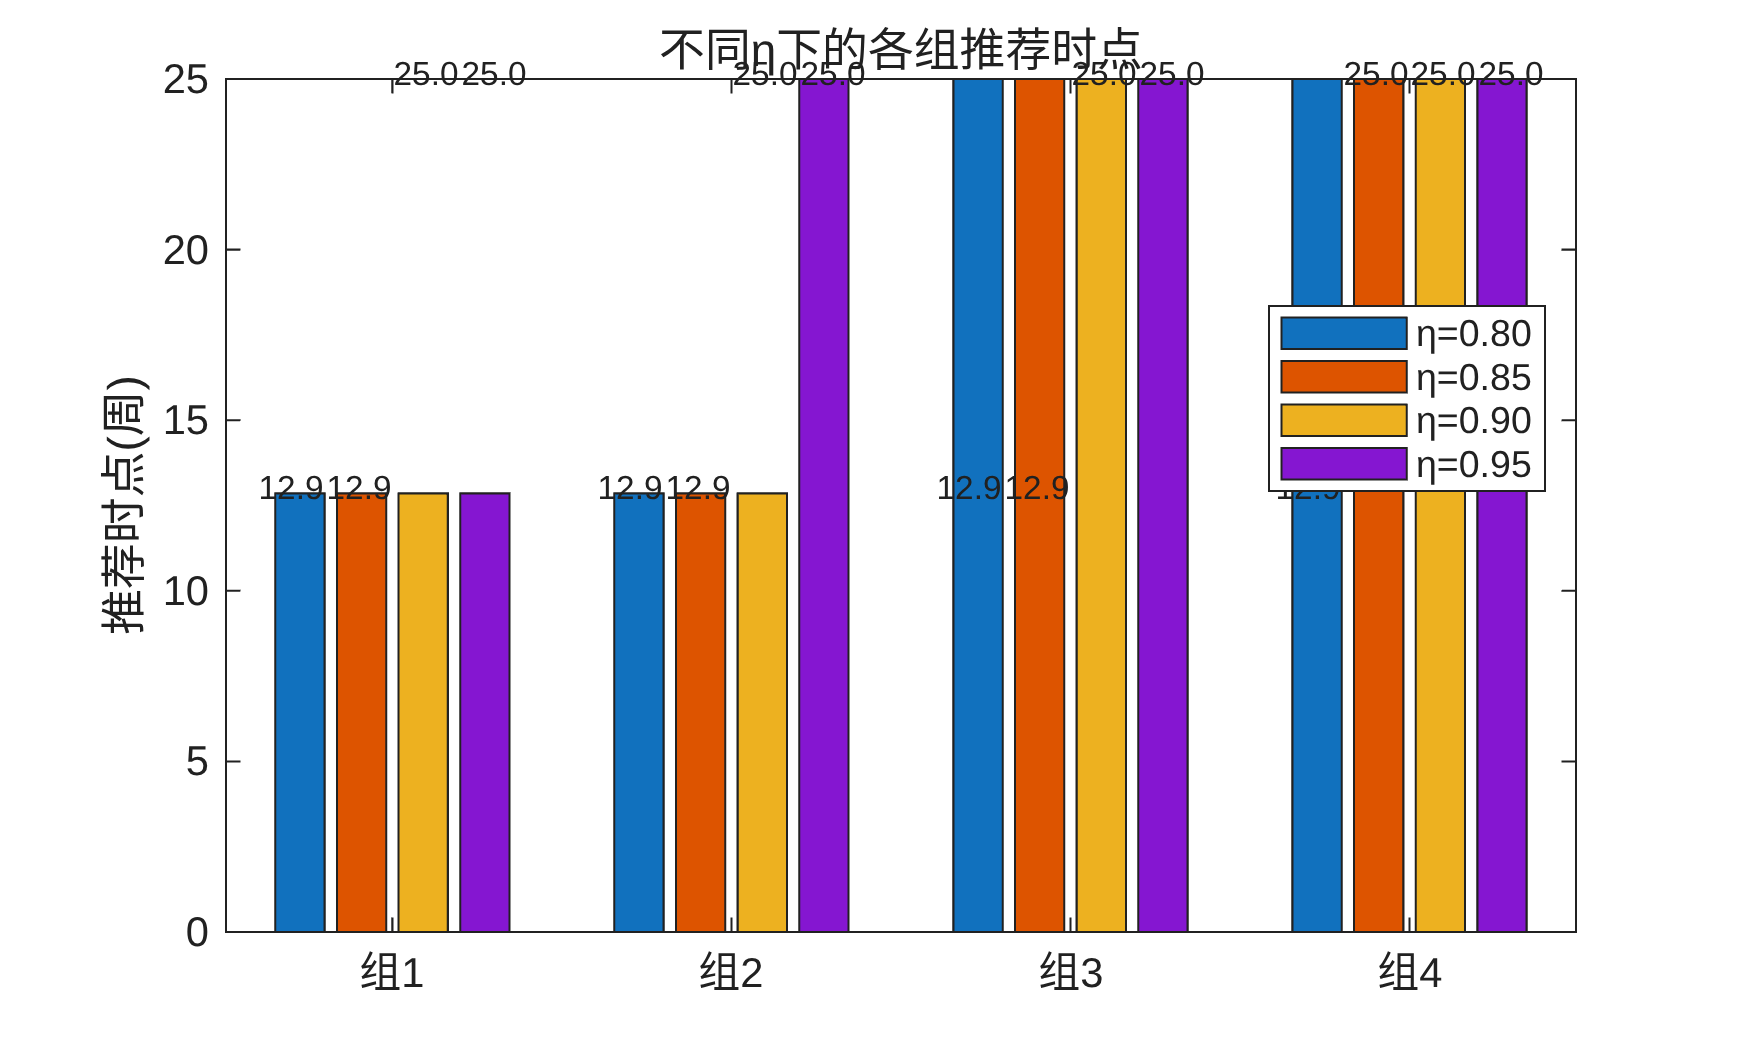
\includegraphics[width=0.72\textwidth]{sens_eta.png}
\caption{达标比例约束 $\eta$ 的灵敏度分析}
\label{fig:senseta}
\end{figure}

检测误差标准差的灵敏度结果见表 \ref{tab:senssigma}. 当 $\sigma$ 缩小为 0.5 倍时，四组均可在 12.86 周达到较高达标比例；当 $\sigma$ 扩大为 2 倍时，四组推荐时点均为 25 周，且达标比例降至 0.751 至 0.788。图 \ref{fig:senssigma} 显示，问题三结果对检测误差设定较敏感。

\begin{table}[H]
\centering
\caption{检测误差标准差变化下的问题三推荐时点}
\label{tab:senssigma}
\begin{tabular}{crrrrr}
\toprule
$\sigma$ 缩放 & 组1/周 & 组2/周 & 组3/周 & 组4/周 & 达标比例范围 \\
\midrule
0.5 & 12.86 & 12.86 & 12.86 & 12.86 & 0.950--0.991 \\
1.0 & 12.86 & 12.86 & 12.86 & 25.00 & 0.879--0.908 \\
2.0 & 25.00 & 25.00 & 25.00 & 25.00 & 0.751--0.788 \\
\bottomrule
\end{tabular}
\end{table}

\begin{figure}[H]
\centering
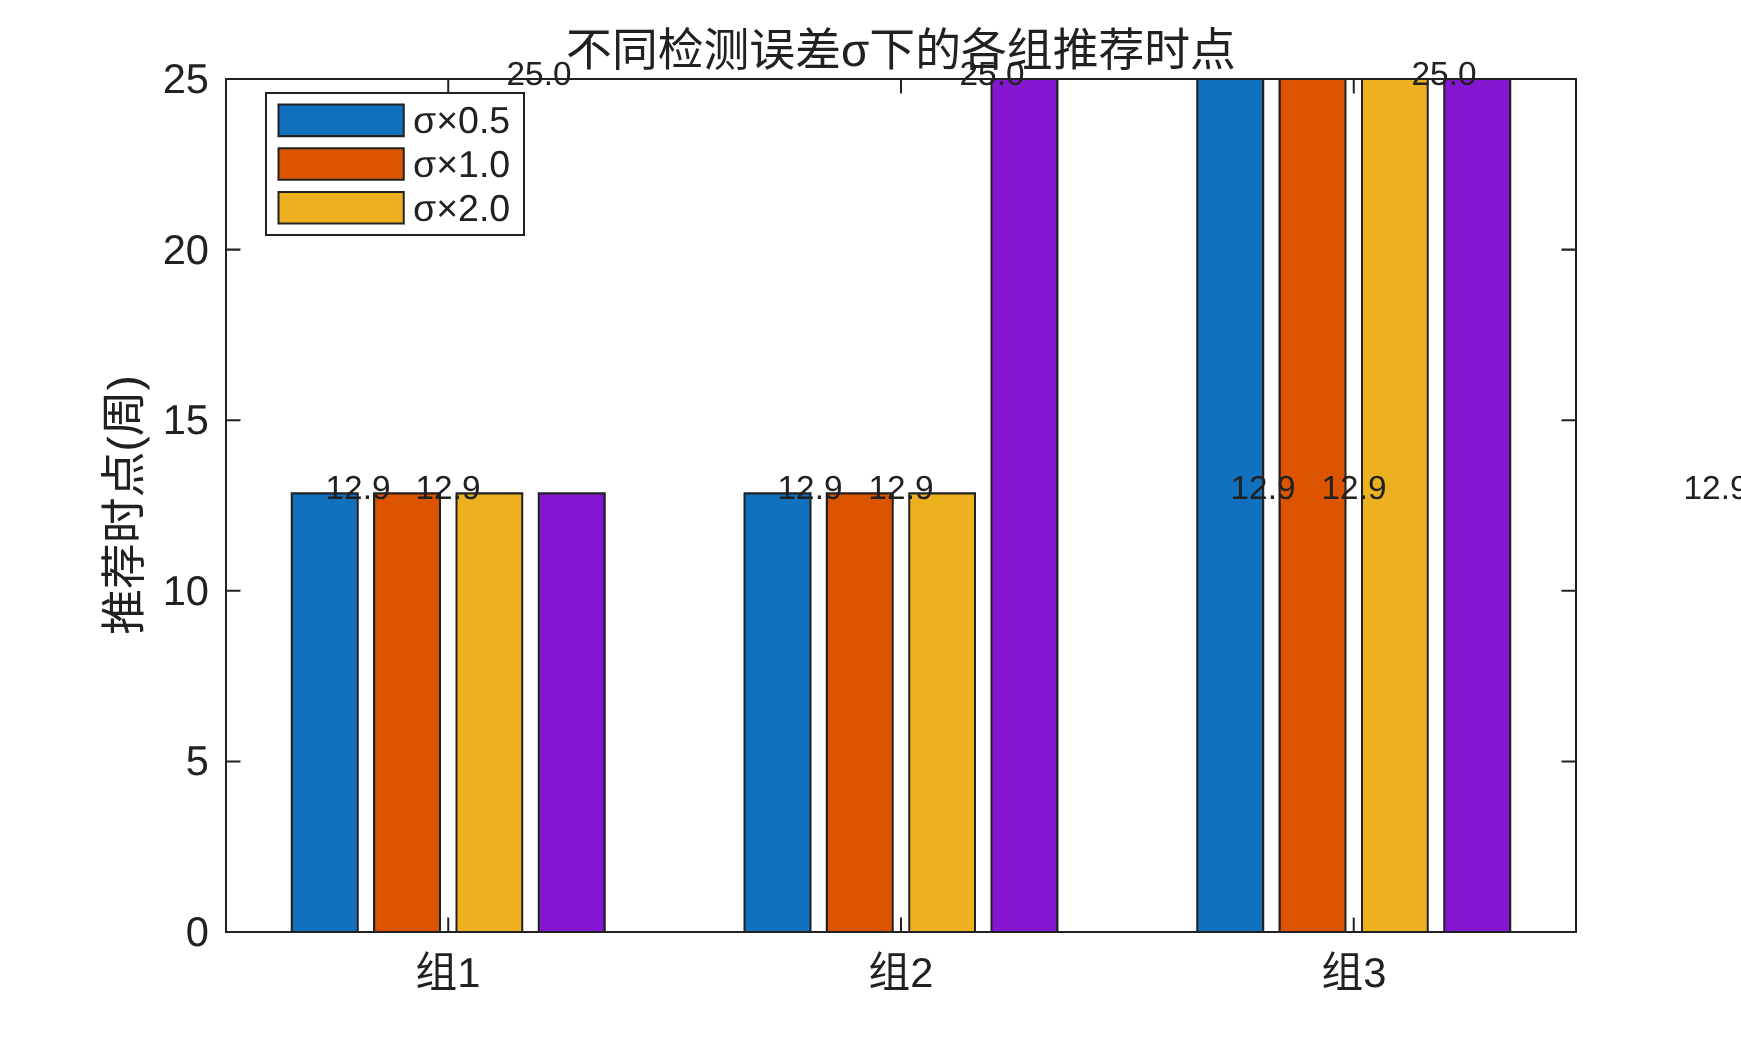
\includegraphics[width=0.72\textwidth]{sens_sigma.png}
\caption{检测误差标准差的灵敏度分析}
\label{fig:senssigma}
\end{figure}

\section{问题四：女胎染色体异常综合判定}

\subsection{异常标签与评分指标}

女胎样本不能使用 Y 染色体浓度，因此本文以“染色体的非整倍体”字段构造异常标签。605 条女胎记录中，异常样本 67 条，正常样本 538 条。异常类型分布中，T18 相关记录较多，类别不平衡会影响模型评价，因此后续同时报告准确率、召回率、精确率和 F1 值。

构造 6 类异常评分分量：
\begin{equation}
D_{13}=\widetilde{|Z_{13}|},\quad
D_{18}=\widetilde{|Z_{18}|},\quad
D_{21}=\widetilde{|Z_{21}|},\quad
D_X=\widetilde{|Z_X|},
\end{equation}
\begin{equation}
D_{GC}=\widetilde{|GC-\overline{GC}|}.
\end{equation}
其中 $\widetilde{\cdot}$ 表示 min-max 归一化。读段质量风险定义为
\begin{equation}
D_{read}=\frac{1}{5}\left[(1-\widetilde{L})+(1-\widetilde{M})+\widetilde{N}+(1-\widetilde{O})+\widetilde{AA}\right],
\end{equation}
其中 $L$ 为原始读段数，$M$ 为比对比例，$N$ 为重复读段比例，$O$ 为唯一比对读段数，$AA$ 为过滤比例。读段数、比对比例和唯一比对读段数越低，质量风险越高；重复读段比例和过滤比例越高，质量风险越高。

\subsection{综合异常评分与阈值选择}

主模型采用等权综合异常评分：
\begin{equation}
S_i=\frac{1}{6}(D_{13,i}+D_{18,i}+D_{21,i}+D_{X,i}+D_{GC,i}+D_{read,i}).
\end{equation}
PCA 权重作为对比方案，其权重见表 \ref{tab:q4weight}. 等权方案便于解释，PCA 方案用于检查权重设定是否显著改变分类效果\cite{jolliffe2002}。

\begin{table}[H]
\centering
\caption{女胎异常评分分量权重}
\label{tab:q4weight}
\begin{tabular}{lrr}
\toprule
分量 & 等权权重 & PCA 权重 \\
\midrule
$|Z_{13}|$ & 0.1667 & 0.2070 \\
$|Z_{18}|$ & 0.1667 & 0.2037 \\
$|Z_{21}|$ & 0.1667 & 0.0478 \\
$|Z_X|$ & 0.1667 & 0.1847 \\
GC 偏离 & 0.1667 & 0.1947 \\
读段质量风险 & 0.1667 & 0.1621 \\
\bottomrule
\end{tabular}
\end{table}

设异常判定阈值为 $\theta$：
\begin{equation}
\hat{A}_i=
\begin{cases}
1,&S_i\ge \theta,\\
0,&S_i<\theta.
\end{cases}
\end{equation}
主阈值通过 Youden 指数选择\cite{youden1950}：
\begin{equation}
J(\theta)=Sensitivity(\theta)+Specificity(\theta)-1.
\end{equation}
同时设置偏召回阈值，使召回率尽量达到 0.90 以上，用于减少异常样本漏判。

图 \ref{fig:q4score} 展示正常与异常样本异常评分的分布。两类样本存在重叠，说明单一综合评分的判别能力有限；阈值降低可以减少漏判，但会带来更多假阳性。

\begin{figure}[H]
\centering
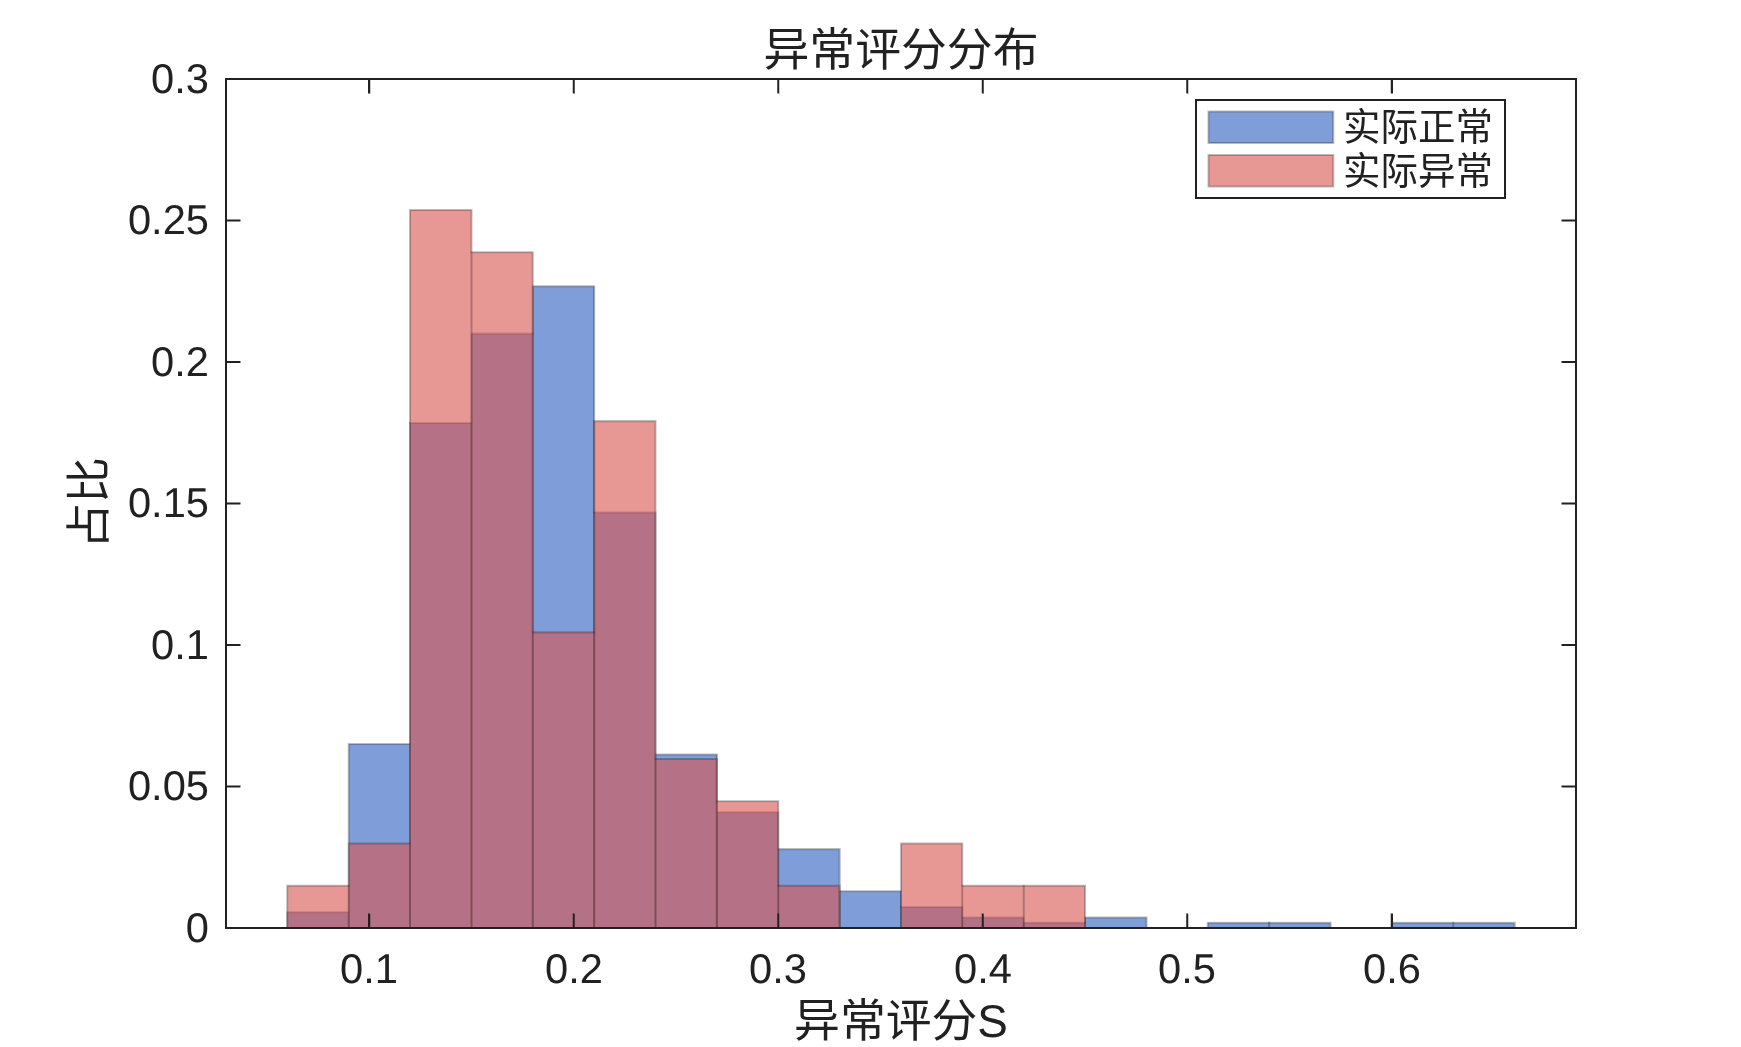
\includegraphics[width=0.72\textwidth]{q4_score_hist.png}
\caption{女胎异常评分分布}
\label{fig:q4score}
\end{figure}

图 \ref{fig:q4threshold} 给出 F1 与 Youden 指数随阈值变化的曲线。Youden 主阈值为 0.2111，偏召回阈值为 0.1293，PCA 权重方案阈值为 0.1182。

\begin{figure}[H]
\centering
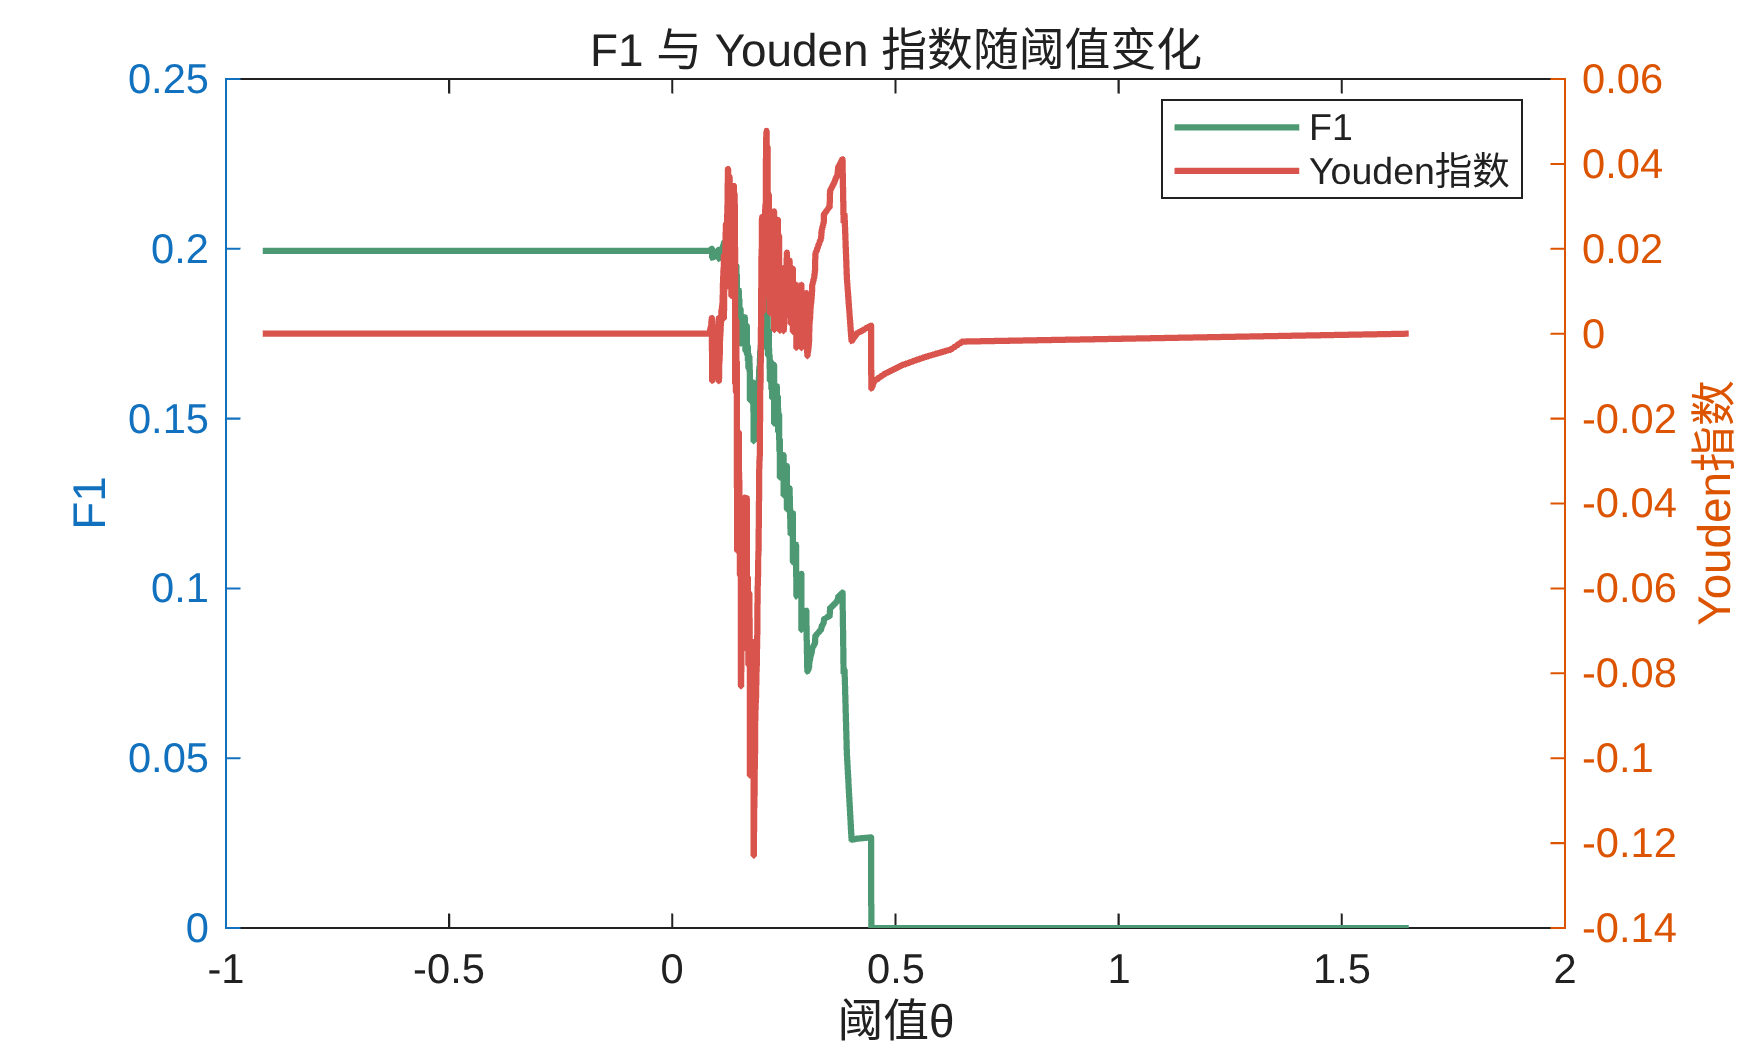
\includegraphics[width=0.72\textwidth]{q4_threshold_curve.png}
\caption{女胎异常判定阈值曲线}
\label{fig:q4threshold}
\end{figure}

\subsection{判定结果与评价}

表 \ref{tab:q4metrics} 给出三种方案的评价指标。Youden 主阈值下准确率为 0.653，但召回率仅为 0.358，不适合单独作为低漏判筛查规则。偏召回阈值将召回率提升到 0.910，PCA 权重方案召回率达到 0.940，但两者精确率均约为 0.11，说明假阳性较多。对于产前筛查任务，低漏判方案可作为进一步检查的提示规则，但不能作为确诊依据。

\begin{table}[H]
\centering
\caption{女胎异常判定评价指标}
\label{tab:q4metrics}
\begin{tabular}{lrrrrr}
\toprule
方案 & 阈值 & 准确率 & 召回率 & 精确率 & F1 \\
\midrule
等权评分（Youden） & 0.2111 & 0.653 & 0.358 & 0.126 & 0.186 \\
等权评分（偏召回） & 0.1293 & 0.207 & 0.910 & 0.114 & 0.203 \\
PCA 权重评分 & 0.1182 & 0.203 & 0.940 & 0.116 & 0.207 \\
\bottomrule
\end{tabular}
\end{table}

Youden 主阈值对应的混淆矩阵见图 \ref{fig:q4cm}. 异常样本数量少，且异常与正常评分重叠较多，因此精确率偏低。论文结论中将该模型定位为辅助筛查方法，更符合数据表现。

\begin{figure}[H]
\centering
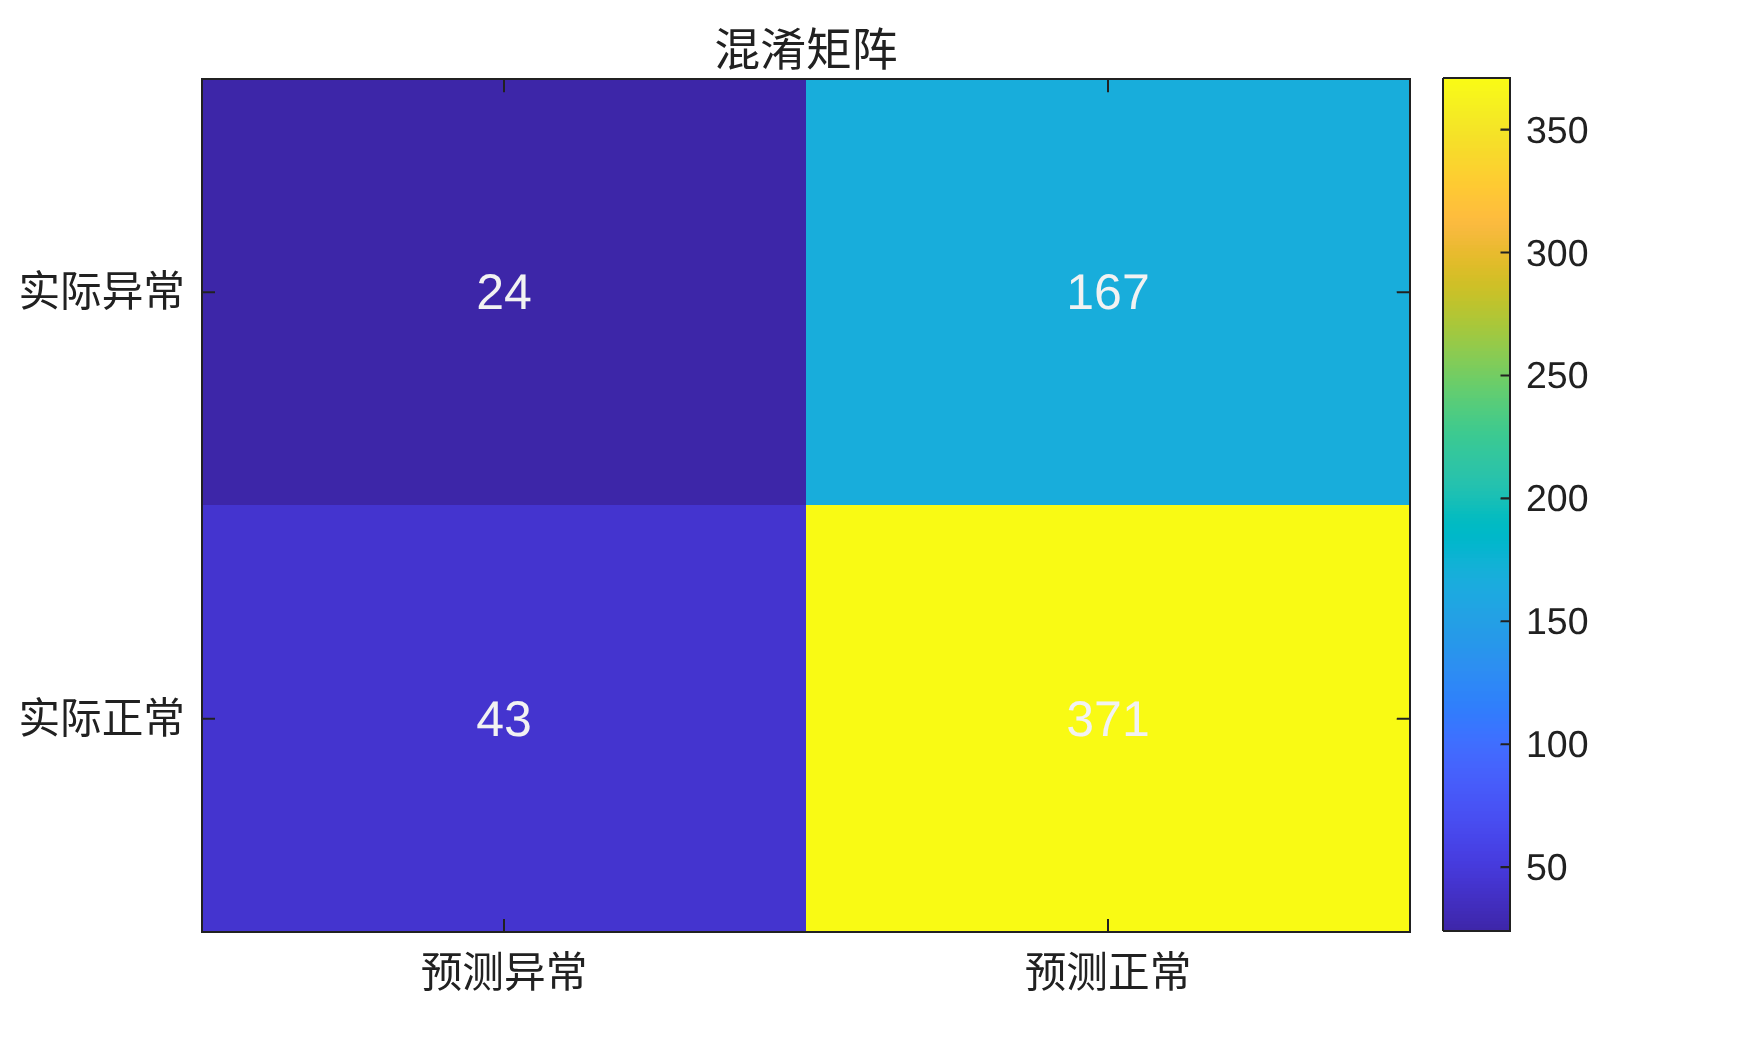
\includegraphics[width=0.62\textwidth]{q4_cm_heatmap.png}
\caption{Youden 主阈值下的女胎异常判定混淆矩阵}
\label{fig:q4cm}
\end{figure}

\subsection{异常类型判定与 BMI 分层}

对被判为异常的样本，进一步构造类型评分：
\begin{equation}
S_{13}=\widetilde{|Z_{13}|}+\rho\widetilde{|GC_{13}-\overline{GC}_{13}|},
\end{equation}
\begin{equation}
S_{18}=\widetilde{|Z_{18}|}+\rho\widetilde{|GC_{18}-\overline{GC}_{18}|},\qquad
S_{21}=\widetilde{|Z_{21}|}+\rho\widetilde{|GC_{21}-\overline{GC}_{21}|}.
\end{equation}
本文取 $\rho=1$。若第二高类型评分不低于最高评分的 0.8 倍，则判为复合异常。Youden 主阈值下共预测 T13 12 条、T18 67 条、T21 53 条、T13T18 20 条、T13T21 5 条、T18T21 26 条、T13T18T21 8 条。改变 $\rho$ 为 0.5 或 2 时，T18 和复合异常数量有所变化，但主要类型分布仍以 T18 和 T21 相关预测为主。

BMI 不直接进入异常评分，而用于分层评价。按有效 BMI 四分位数分为四层后，各层漏判率分别为 0.545、0.474、0.774、0.667，误判率分别为 0.321、0.295、0.275、0.345。第三层漏判率较高，第四层误判率较高，说明 BMI 水平可能影响异常评分的稳定性。后续若有更多样本，可进一步在不同 BMI 层中单独校准阈值。

\section{模型检验}

为保证模型和代码实现的一致性，本文对数据规模、特殊值、数学一致性和稳定性进行了检查。全量数据检查确认男胎记录数为 1082、女胎记录数为 605、男胎孕妇数为 267、女胎孕妇数为 147；男胎 Y 浓度达标标签严格来自 $Y\ge0.04$，女胎异常标签来自 AB 列而非出生健康结果列。

特殊值检验覆盖孕周解析、$Y=0.04$ 达标边界、女胎 T13/T18/T21 标签构造和切点搜索手算样例。数学一致性检验在真实数据子集上验证了相关系数维度、回归系数维度、风险函数分段、达标比例范围和阈值评价指标。稳定性检验显示，确定性切点搜索 10 次结果完全一致；蒙特卡洛扰动在固定随机种子下可复现。

交叉验证方面，将切点搜索步长由 2 调整为 1 后，总风险不劣于粗步长，最佳时点差异不超过 0.3 周；将时点网格由按天枚举改为 0.5 周网格后，推荐时点差异不超过 0.55 周。本文未使用迭代优化算法，核心搜索为有限枚举和阈值遍历，因此不存在迭代收敛问题。

\section{模型评价}

\subsection{模型优点}

本文模型具有以下优点。
\begin{enumerate}
  \item 建模链条完整。问题一到问题三从浓度关系分析逐步过渡到 BMI 分组和检测时点优化，问题四针对女胎缺少 Y 染色体信息的特点单独构造异常评分，四问之间逻辑连续。
  \item 数据口径清晰。回归估计使用记录层数据，分组优化使用孕妇层数据，既保留多次检测信息，又避免重复检测个体在分组决策中过度加权。
  \item 决策模型可解释。风险函数由时间风险和不达标惩罚组成，BMI 切点通过有序枚举获得，推荐时点能直接对应到组内达标比例和总风险。
  \item 误差分析较充分。问题二使用蒙特卡洛扰动考察检测误差，问题三通过正态达标概率显式引入检测误差，并对 $\eta$、$\sigma$、$\lambda$ 和 $\rho$ 等参数进行灵敏度分析。
  \item 女胎判定避免单一准确率评价。模型同时报告召回率、精确率和 F1 值，并给出偏召回阈值，能反映异常样本不平衡下的漏判风险。
\end{enumerate}

\subsection{模型不足}

本文模型仍存在以下限制。
\begin{enumerate}
  \item 问题一主模型虽然整体显著，但 $R^2$ 仅为 0.0636，说明 Y 染色体浓度的大部分个体波动尚未被现有变量解释。
  \item 同一孕妇的多次检测记录在回归模型中按独立记录处理，未显式建立个体随机效应结构，可能低估重复检测带来的相关性。
  \item 首次达标时间只能由观测到的检测时点近似得到，若真实达标发生在两次检测之间，则观测首次达标时间可能偏晚。
  \item 问题三高 BMI 组推荐时点达到 25 周上界，该结果受候选时点范围和可靠性约束影响较大，不宜解释为所有高 BMI 孕妇均应等待至 25 周。
  \item 女胎异常样本仅 67 条，且综合评分在正常与异常样本之间存在较大重叠。阈值在全样本上选取，评价指标可能偏乐观，模型更适合作为辅助筛查规则。
\end{enumerate}

\subsection{改进方向}

若后续获得更完整的纵向检测数据，可在男胎 Y 染色体浓度模型中引入孕妇个体效应或删失达标时间模型，减少重复检测独立性假设带来的偏差。对于 NIPT 时点选择，可结合真实临床损失、复检成本和孕妇风险偏好重新校准 $C(t)$ 与 $\lambda$。对于女胎异常判定，可在更多异常样本基础上划分训练集和验证集，或按 BMI 层、孕周层建立分层阈值，以降低全样本阈值带来的过拟合风险。

\section{结论}

本文围绕 2025 年 C 题 NIPT 检测时点选择与胎儿异常判定问题，建立了基于回归分析、BMI 有序分组、风险最小化和综合评分的模型体系。

问题一结果表明，男胎 Y 染色体浓度与孕周显著正相关，与 BMI、年龄、体重显著负相关。交互项回归模型整体显著，残差标准差为 0.0325，但 $R^2$ 较低，说明该模型适合刻画总体趋势和误差水平，不适合过度解释单个样本浓度。

问题二在仅考虑 BMI 的设定下，将 267 名男胎孕妇分为 4 个连续 BMI 区间。BMI 不超过 30.05 的前三组推荐 10 周检测，高 BMI 组推荐 12.29 周检测。检测误差蒙特卡洛分析和 $\lambda$ 灵敏度分析均显示该结论较稳定。

问题三加入年龄、孕情、妊娠方式、测序质量和检测误差后，推荐时点整体后移。前三组推荐 12.86 周，高 BMI 组推荐 25 周。该结果提示，在要求较高达标概率时，检测误差和个体差异会显著提高过早检测风险；同时，高 BMI 组触及候选上界，需要结合临床可接受窗口谨慎使用。

问题四针对女胎缺少 Y 染色体指标的情况，构造了 6 分量综合异常评分。Youden 主阈值下准确率为 0.653、召回率为 0.358；偏召回阈值可将召回率提升至 0.910，但精确率仅为 0.114。该模型可用于低漏判倾向的辅助筛查，不应作为最终诊断依据。

\clearpage
\begin{thebibliography}{99}
\bibitem{contest2025c} 全国大学生数学建模竞赛组委会. 2025 年高教社杯全国大学生数学建模竞赛 C 题：NIPT 的时点选择与胎儿异常判定[Z]. 2025.
\bibitem{lo1997} Lo Y M D, Corbetta N, Chamberlain P F, et al. Presence of fetal DNA in maternal plasma and serum[J]. Lancet, 1997, 350(9076): 485--487.
\bibitem{bianchi2014} Bianchi D W, Parker R L, Wentworth J, et al. DNA sequencing versus standard prenatal aneuploidy screening[J]. New England Journal of Medicine, 2014, 370(9): 799--808.
\bibitem{hui2020} Hui L, Bianchi D W. Fetal fraction and noninvasive prenatal testing: what clinicians need to know[J]. Prenatal Diagnosis, 2020, 40(2): 155--163.
\bibitem{deng2022} Deng C, Liu S. Factors affecting the fetal fraction in noninvasive prenatal screening: a review[J]. Frontiers in Pediatrics, 2022, 10: 812781.
\bibitem{montgomery2012} Montgomery D C, Peck E A, Vining G G. Introduction to Linear Regression Analysis[M]. 5th ed. Hoboken: John Wiley \& Sons, 2012.
\bibitem{jolliffe2002} Jolliffe I T. Principal Component Analysis[M]. 2nd ed. New York: Springer, 2002.
\bibitem{youden1950} Youden W J. Index for rating diagnostic tests[J]. Cancer, 1950, 3(1): 32--35.
\end{thebibliography}

\clearpage
\appendix
\renewcommand{\thesection}{附录\Alph{section}}
\renewcommand{\thesubsection}{\thesection.\arabic{subsection}}
\titleformat{\section}{\centering\heiti\zihao{3}}{\thesection}{1em}{}
\titleformat{\subsection}{\heiti\zihao{4}}{\thesubsection}{0.8em}{}
\section{程序与结果文件说明}

本文代码和结果位于 `2025c建模代码材料' 目录中。主程序为 `src/main\_2025C.m'，依次调用数据读取、预处理、问题一至问题四模型函数和灵敏度分析函数。最终结果表位于 `outputs/tables'，图件位于 `figures'。代码一致性测试文件为 `tests/test\_2025C.m'，测试日志显示全部测试通过。为便于论文附录查阅，已将最终交付源码复制到 `2025C论文/paper/code'，下面给出完整求解代码。

论文正文使用的主要图件已复制到 `2025C论文/paper/figures'，包括问题一散点图和残差图、问题二 BMI 分组和风险曲线、问题三推荐时点对比和灵敏度分析图、问题四异常评分分布和混淆矩阵图。

\section{完整程序代码}

\subsection{主程序 main\_2025C.m}
\VerbatimInput{code/main_2025C.m}

\subsection{数据读取 load\_data.m}
\VerbatimInput{code/load_data.m}

\subsection{数据预处理 preprocess\_data.m}
\VerbatimInput{code/preprocess_data.m}

\subsection{最小二乘回归 func\_ols.m}
\VerbatimInput{code/func_ols.m}

\subsection{有序 BMI 切点搜索 func\_cutsearch.m}
\VerbatimInput{code/func_cutsearch.m}

\subsection{问题一 q1\_correlation\_regression.m}
\VerbatimInput{code/q1_correlation_regression.m}

\subsection{问题二 q2\_bmi\_group\_timing.m}
\VerbatimInput{code/q2_bmi_group_timing.m}

\subsection{问题三 q3\_multifactor\_timing.m}
\VerbatimInput{code/q3_multifactor_timing.m}

\subsection{问题四 q4\_female\_abnormal\_judge.m}
\VerbatimInput{code/q4_female_abnormal_judge.m}

\subsection{灵敏度分析 sensitivity\_analysis.m}
\VerbatimInput{code/sensitivity_analysis.m}

\subsection{图件导出 fig\_export.m}
\VerbatimInput{code/fig_export.m}

\end{document}
